%Version 3 December 2023 modified by Douwe to suit style of thesis proposal

\documentclass[iicol,pdflatex,sn-mathphys-ay]{sn-jnl}% Math and Physical Sciences Author Year Reference Style

%%%% Standard Packages
\usepackage{graphicx}%
\usepackage{multirow}%
\usepackage{amsmath,amssymb,amsfonts}%
\usepackage{amsthm}%
\usepackage{mathrsfs}%
\usepackage[title]{appendix}%
\usepackage{xcolor}%
\usepackage[table]{xcolor}
\usepackage{textcomp}%
\usepackage{manyfoot}%
\usepackage{booktabs}%
\usepackage{algorithm}%
\usepackage{algorithmicx}%
\usepackage{algpseudocode}%
\usepackage{listings}%


%extra packages added by Douwe:
\usepackage{fix-cm} % to ensure all fonts are supported
\usepackage{tabularx}
\usepackage{mdframed} %using this I can insert textboxes
\usepackage{placeins} %\usepackage[above,below]{placeins} % creates float barriers after every section
\usepackage{natbib} % for concise bibliography
\usepackage{caption}
\captionsetup[figure]{skip=3pt} % distance between a figure/table and its caption
\usepackage{hyperref} %needs to be the last package that is imported!!!
%%%%

%%%%%=============================================================================%%%%
%%%%  Remarks: This template is provided to aid authors with the preparation
%%%%  of original research articles intended for submission to journals published 
%%%%  by Springer Nature. The guidance has been prepared in partnership with 
%%%%  production teams to conform to Springer Nature technical requirements. 
%%%%  Editorial and presentation requirements differ among journal portfolios and 
%%%%  research disciplines. You may find sections in this template are irrelevant 
%%%%  to your work and are empowered to omit any such section if allowed by the 
%%%%  journal you intend to submit to. The submission guidelines and policies 
%%%%  of the journal take precedence. A detailed User Manual is available in the 
%%%%  template package for technical guidance.
%%%%%=============================================================================%%%%%

%\raggedbottom %makes all pages the height of the text on that page. No extra vertical space is added. See also Document Styles.

%%\unnumbered% uncomment this for unnumbered level heads

\begin{document}
\begin{titlepage}
    \thispagestyle{empty}
    \begin{center}
        \vspace*{2cm} % Adjust this to position content vertically
        {\huge \textsc{Wageningen University}}\\
        \vspace{1cm}% 1cm?
        {\Large \textsc{Hydrology and Environmental Hydraulics Group}}\\
        \vspace{1cm} % 8mm
        {\large \textsc{Master Thesis}}\\
        \vspace{5mm}
        {\large \textsc{Earth and Environment}}\\
        \vspace*{2cm}
        \rule{.8\linewidth}{.6pt}\\[0.6cm]
        \begin{minipage}{0.8\linewidth}
            \centering
            {\Huge \bfseries A comparison of Markov Chain Monte Carlo algorithms for parameter calibration in hydrology}
        \end{minipage}\\[0.4cm]
        \rule{.8\linewidth}{.6pt}\\[2cm]%2.5cm
        \textit{Author:}\\
        Douwe Kamper\\
        \vspace*{0.5cm}
        \textit{Supervisors:}\\
        Lieke Melsen, Syed Mustafa \& Shota Gugushvili\\
        \vspace{0.5cm} 
        \today % Date
    \end{center}
    \vspace*{1cm} % 1.5cm
    \begin{center}
        \includegraphics[scale=0.45]{Figures/logo.jpg}
    \end{center}
\end{titlepage}
\newpage

\section*{Abstract}\label{abstract}
Calibration of model parameters is key for improving the reliability of model predictions and thereby informed decision making. Markov Chain Monte Carlo (MCMC) is a statistical method that has found widespread application in hydrological modelling for calibrating parameters and quantifying their uncertainty. Hundreds of MCMC algorithms have been designed, yet only a small selection is used by hydrologists, excluding some of the most popular algorithms in other fields of science, despite the absence of a comprehensive benchmark supporting this decision. In this study a contribution is made towards this benchmark, by comparing a single algorithm popular outside hydrology (Goodman and Weare’s Affine Invariant sampler; AI) to two algorithms popular in hydrology (Ter Braak’s DE and DE-SNK). Four simple steady-state synthetic groundwater flow models (developed using MODFLOW 6) were calibrated, with the number of calibrated parameters ranging from one to five. Performance diagnostics suggest that all three algorithms converge to the same posterior distribution for all models, but AI is distinctly less efficient than the others. DE-SNK overtakes DE for the model with the most calibrated parameters and is therefore recommended for groundwater modelling in general. In contrast, existing literature, based on vadose zone modelling, recommends AI based strategies below 10 calibrated parameters, implying the need to further study under which conditions which algorithm outperforms the others. 

%word count = 186 for Draft, 216 for Final
%%% problem description 
%Markov Chain Monte Carlo (MCMC) is a statistical method that has found widespread application in hydrological modelling for calibrating parameters and quantifying their uncertainty. Hundreds of MCMC algorithms have been designed, yet only a small selection is used by hydrologists, excluding some of the most popular algorithms in other fields of science, while a comprehensive benchmark supporting this decision does not exist. 
%%% objective
%In this study a contribution is made towards this comprehensive benchmark by
%%%methods
%comparing a single algorithm popular outside hydrology (Goodman and Weare’s Affine Invariant sampler, AI) to two algorithms popular inside hydrology (Ter Braak’s DE and DE-SNK). Four simple synthetic groundwater flow models (MODFLOW 6) were calibrated with the number of calibrated parameters ranging from 1 to 5. % also vary priors and likelihoods
%%% results
%Performance diagnostics suggest that all three algorithms converge to the same posterior distribution for all models, but AI is distinctly less efficient than the others. DE-SNK overtakes DE for the model with the most calibrated parameters 
%%% conclusion
%and is therefore recommended for groundwater modelling.
%%% outlook
%In contrast, existing literature, based on vadose zone modelling, recommends AI based strategies below 10 calibrated parameters, implying the need for further research. 







\section{Introduction}\label{sec1}
Model predictions are at the heart of hydrological decision making, they for instance quantify the effect of groundwater abstraction on groundwater levels. An essential step to improve model predictions is calibration of the model parameters. Conventionally, calibration refers to the process of tuning model parameters to optimize the similarity between observed and simulated values, with the objective to find a unique set of optimal parameters, e.g. \cite{refsgaard1997parameterisation}, where the performance of a parameter set is evaluated with a goodness of fit diagnostic such as the Kling-Gupta Efficiency \citep{gupta2009decomposition}. This is a challenging problem to solve, as the parameter space of hydrological models is characterized by many local optima (sometimes hundreds), which are not necessarily close to the global optimum \citep{duan1992effective}. Historically, local calibration methods such as the widely used Levenberg-Marquardt algorithm \citep{beven1992future} have been used for this purpose. Although computationally efficient, these local calibration methods do not attempt to explore all probable parts of parameter space. As a consequence, these local methods often converge to a local optimum, rather than the global optimum \citep{hendrickson1988comparison, blasone2007parameter}. Therefore, it is often recommended to restart optimization from different starting points multiple times, in the hope of arriving at a better optimum. However, if there are many local optima, this strategy is unlikely to succeed, while increasing the computational burden. Global search algorithms have been developed to avoid this problem, at the cost of generally being much slower. A prominent example is the Shuffled Complex Evolution (SCE-UA) method developed at the University of Arizona by \cite{duan1992effective}. 
%Global search methods have been developed to overcome this limitation by probabilistically or systematically exploring the parameter space to locate the global optimum, even in the presence of many local optima. These methods, such as genetic algorithms, simulated annealing, or evolutionary strategies, often rely on stochastic or heuristic techniques and are typically slower but more robust than local methods.

When making decisions based on model predictions, not only the prediction itself is important (global optimum), but also its uncertainty. For some purposes, such as flood forecasting, the uncertainty estimate may even be more important than the prediction itself. Although SCE-UA can reliably find the global optimum, it is inapplicable for parameter uncertainty assessment \citep{vrugt2003shuffled} due to its deterministic rather than probabilistic nature \citep{vrugt2006application}. \cite{vrugt2003shuffled} addressed this by integrating SCE-UA into a probabilistic statistical method called Markov Chain Monte Carlo (MCMC), creating the Shuffled Complex Evolution Metropolis algorithm (SCEM-UA). 

\begin{table*}[hbt!]
\caption{A comparison of the popularity of several MCMC algorithms between all fields of science and hydrology specifically. Popularity is quantified by counting how often the paper introducing the specific algorithms is cited. Three hydrological journals have been selected to indicate the popularity in hydrology: Journal of hydrology, Water Resources Research \& Advances in Water Resources.  These are the three journals where MCMC methods are most discussed, while  specifically tailored to hydrology (\hyperref[appendix search strat]{\textcolor{blue}{Appendix }\ref{appendix search strat}}).}
\label{tab1}
\begin{tabularx}{\textwidth}{lXXl} 
    \toprule
    MCMC Method & citation in all journals & citations in hydrological journals & paper introducing algorithm\\
    \midrule
    %Metropolis & 23718 & 174 & \cite{metropolis1953equation}\\ % remove?
    Metropolis-Hastings & 7922 & 123 & \cite{hastings1970monte}\\
    Differential Evolution (DE) & 565 & 32 & \cite{terbraak2006markov}\\
    DE with snooker updater (DE-SNK) & 338 & 53 & \cite{terbraak2008differential}\\
    DREAM & 777 & 196 & \cite{vrugt2009accelerating}\\
    Multiple-Try DREAM\textsubscript{(zs)} & 360 & 93\phantom{0} & \cite{laloy2012high}\\
    Affine Invariant sampler (AI) & 1903 & 9\phantom{0}\phantom{0} & \cite{goodman2010ensemble} \\
    Hamiltonian Monte Carlo (HMC) & 2154 & 10\phantom{0} & \cite{duane1987hybrid}\\
    No-U-Turn Sampler (NUTS) & 1886 & 17\phantom{0} & \cite{hoffman2014no}\\ 
    \bottomrule
\end{tabularx}
\end{table*}

The advantage of MCMC with regard to parameter uncertainty estimation is that MCMC produces a probability distribution for each parameter, referred to as the posterior. Traditional MCMC algorithms such as Metropolis-Hastings achieve this as follows. Prior knowledge is formalized into a prior probability distribution for each parameter. Additionally, a likelihood function is selected, which quantifies the probability of the observed data given the (sampled) parameter value(s) of the hydrological model. 
%From now on, methods differ depending on the selected MCMC algorithm, here is described how methods similar to the first MCMC algorithm work \citep{metropolis1953equation}. 
With the prior and likelihood defined, sampling can start. 
For each parameter an initial value is determined from which step-wise exploration of parameter space starts. New locations are generated by a proposal distribution and accepted or rejected stochastically, based on an acceptance ratio, which is calculated with the prior and likelihood of the sampled parameter values. These subsequent dependent steps form a Markov chain. 
% Note that more advanced MCMC algorithms exist, that work quite differently. 
Sampling is conventionally split into two phases: during the burn-in phase the chain searches for the most probable areas of the parameter space and during the main sampling phase this area has been reached and is explored. Sampling is generally stopped when some arbitrary threshold of a selected convergence diagnostic is reached. The estimated posterior probability distribution is the distribution formed by by collecting all locations the Markov chain has sampled during the main sampling phase, where the probability equals the relative sampling density. The success of a MCMC algorithm largely depends on whether its chain(s) get stuck in a subspace and on the speed by which they converge to this distribution. % finish of by saying that MCMC become increasingly relevant due to advances in computational power and additionally some algorithms being easily paralizable for use on HPC cluster (MT-DREAM ref, emcee ref). 

Since the inception of MCMC with Random Walk Metropolis \citep{metropolis1953equation}, hundreds of MCMC algorithms have been developed and introduced in scientific literature \citep{brooks2011handbook}. Two of these algorithms are very popular in hydrological literature (\hyperref[tab1]{\textcolor{blue}{Table} \ref*{tab1}}): Metropolis-Hastings and Differential Evolution Adaptive Metropolis (DREAM). Metropolis-Hastings was developed by \cite{hastings1970monte} and has an asymmetric proposal distribution and modified acceptance probability. \cite{hastings1970monte} solved the issue Random Walk Metropolis has with undersampling of parameter values near a parameter bound, which is caused by parameter bounds only being accessible from one side of the bound. The Metropolis-Hastings proposal distribution approaches a symmetric distribution far from parameter bounds and is symmetric in the absence of parameter bounds. It is still very popular due to its simplicity and versatility \citep{robert2004metropolis}. DREAM was developed more recently \citep{vrugt2009accelerating} as a follow-up of SCEM-UA \citep{vrugt2003shuffled}, with an ensemble method called Differential Evolution (DE) as its main building block \citep{terbraak2006markov}. 

Ensemble methods use multiple chains, where each chain is updated using the (current) position of the other chains in the ensemble. \cite{terbraak2008differential} introduced another ensemble algorithm (DE-SNK), which utilises a move called the snooker update in conjunction with the Differential Evolution move, to improve exploration of parameter space. Another powerful ensemble method is the Affine Invariant Ensemble sampler (AI) developed by \cite{goodman2010ensemble}, which is very popular in other disciplines, but almost absent in hydrology (\hyperref[tab1]{\textcolor{blue}{Table} \ref*{tab1}}).

The choice of which MCMC method to use is not a straightforward one to make with the sheer amount of methods available and their respective advantages and disadvantages. Some work has been done on comparing MCMC methods within hydrology. \cite{brunetti2023depth} compared DE, DE-SNK, AI and AI-SNK (AI extended with snooker updater) in several toy problems, a synthetic and one actual case study. They found that ensemble methods are suitable for vadose zone modelling, and recommend (as a guideline) Affine Invariant based samplers below 10 dimensions (i.e. fewer than 10 parameters to be calibrated), Differential Evolution based samplers between 10 and 20 dimensions and discourage both above 20 dimensions. This limited performance of most Ensemble samplers in high dimensions is also recognised by the authors of the Affine Invariant sampler python package emcee \citep{hogg2018data}. Conversely, an Affine Invariant MCMC Ensemble sampler with a particle filter showed good performance in a highly dimensional case study where it was used to infer the real rainfall from both rain and runoff observations \citep{bacci2023comparison}.  Considering Differential Evolution based algorithms: \cite{vrugt2009accelerating} argues that DREAM can efficiently handle problems involving high dimensionality and Multiple-Try DREAM(zs) \citep{laloy2012high} has been specifically created for problems involving high dimensionality, further challenging the poor performance of Ensemble samplers in high dimensions. 

A powerful algorithm called Hamiltonian Monte Carlo \citep{duane1987hybrid}, which is widely considered the most effective approach when dealing with high dimensionality \citep{hogg2018data}, is almost absent from hydrological literature (\hyperref[tab1]{\textcolor{blue}{Table} \ref*{tab1}}). Recently, \cite{bacci2023comparison} compared the performance of Hamiltonian Monte Carlo to the Affine Invariant sampler with a particle filter in the highly dimensional case study described above. \cite{ulzega2023bayesian} argue for the use of Hamiltonian Monte Carlo, while presenting the same case study. 

The No-U-Turn Sampler created by \cite{hoffman2014no} is an extension of Hamiltonian Monte Carlo, providing auto-tuning of the two parameters and preventing the sampler to double back and retrace its steps (hence the name). However, it is rarely used in hydrological literature (\hyperref[tab1]{\textcolor{blue}{Table} \ref*{tab1}}), although it is much more user friendly than Hamiltonian Monte Carlo. In contrast, it is very popular in other fields of science. Additionally, the No-U-Turn Sampler is the main algorithm in the state-of-the-art probabilistic programming framework Stan \citep{carpenter2017stan}. It was used in hydrology by \cite{krapu2022differentiable}, who argue for the use of Hamiltonian Monte Carlo to perform inference for time-varying parameters (which results in a high dimensional problem) in hydrological models, supported by a real world case study, analysing 20 years of streamflow records from the Model Parameter Estimation Experiment \citep{duan2006model}. 

%state knowledge gap 
A rigorous benchmark comparing MCMC algorithms remains absent in hydrology, yet this could aid more robust uncertainty estimation. The benchmarks that do exist either compare a limited number of relevant algorithms, such as \cite{brunetti2023depth} comparing only Ensemble samplers, yet excluding DREAM. And/or they compare algorithms for only a specific case study (which is a specific dimensional problem), leaving the relative performance of the different algorithms as a function of dimensionality undetermined, e.g. \cite{bacci2023comparison}. 

%feasibility
Although it would be interesting to address this scientific gap, by comparing the most popular and powerful MCMC algorithms in hydrology with promising MCMC algorithms from other fields of science in a benchmark of varying dimensionality, this proved unfeasible for a MSc thesis. 
Therefore, the scope was scaled down to comparing an algorithm popular outside hydrology (Goodman and Weare's Affine Invariant sampler), to two algorithms popular in hydrology (Ter Braak's DE and DE-SNK, see \hyperref[tab1]{\textcolor{blue}{Table} \ref*{tab1}}). These three algorithms have the advantage, regarding feasibility, that they can all be implemented with the Python package emcee \citep{foreman2013emcee}. This research is similar to \cite{brunetti2023depth}, but applied to groundwater modelling instead of inverse vadose zone modelling. %These are all Ensemble Samplers, 

The performance of these samplers is evaluated with a calibration exercise, in which each sampler is given an identical calculation budget. The parameters of four steady-state synthetic groundwater flow models (MODFLOW6) are calibrated with a dimensionality ranging from 1 to 5. The importance of prior knowledge for model calibration is investigated by comparing the performance of the samplers using two different priors. Additionally, the number of observations per layer in the groundwater flow models is varied, to gain insight in the optimal number of observations. 

%All three of these algorithms are of similar complexity.
%Where the moves in Ter Braak's algorithms are the main building blocks of DREAM and MT-DREAM respectively, and are thus super relevant. 
In \hyperref[RWM_example]{\textcolor{blue}{Chapter} \ref{RWM_example}} a single step of the Metropolis algorithm is described in detail (selected for its simplicity), adapted from \cite{johnson2022bayes}, to provide the (unfamiliar) reader with some insight in the machinery behind MCMC. In \hyperref[Methods]{\textcolor{blue}{Chapter} \ref{Methods}} the Methodology for comparing the different algorithms is described, followed by the results in \hyperref[results]{\textcolor{blue}{Chapter }\ref{results}}. The results are discussed in \hyperref[Discussion]{\textcolor{blue}{Chapter }\ref{Discussion}}, providing recommendations on which sampler to use at which dimensionality, together with attained insights on how to effectively implement MCMC for hydrogeological model calibration. Finally, \hyperref[Conclusions]{\textcolor{blue}{Chapter }\ref{Conclusions}} wraps everything up with the conclusions. %or hydrogeology? ddd



\section{Theoretical Background}\label{RWM_example}
To understand MCMC it is essential to understand Bayes’ rule (\hyperref[eq1]{\textcolor{blue}{Equation} \ref{eq1}}). Bayes’ rule yields the posterior density (probability density distribution of the parameters, $\theta$, given the data), effectively inverting the likelihood, p(data$|\theta$), through multiplication with the prior distribution, p($\theta$), and division by the marginal likelihood, p(data). The marginal likelihood is obtained by integrating the joint density, p(data, $\theta$), across the range of $\theta$. With each additional parameter, another dimension is added to the integral, quickly becoming unfeasible to solve analytically. This is where MCMC comes in. Since the posterior density is proportional to the likelihood multiplied by the prior (\hyperref[eq2]{\textcolor{blue}{Equation} \ref{eq2}}), the shape of the posterior is known, just not its height. Conveniently only the shape of the posterior is required to sample from it. 

\begin{equation}
p(\theta|data) = \frac{p(data|\theta)p(\theta)}{p(data)}\label{eq1}
\end{equation}

\begin{equation}
p(\theta|data) \propto p(data|\theta)p(\theta)\label{eq2}
\end{equation}
\newline %important for formatting for this specific equation (because it is not in the 'align' environment)
\indent Consider a single parameter model with a Gaussian prior and likelihood. The selected prior for parameter $\theta$ has a mean of zero and standard deviation of one. The prior distribution is given by \hyperref[eq3]{\textcolor{blue}{Equation} \ref{eq3}} and its corresponding probability density function (pdf) is given by \hyperref[eq3b]{\textcolor{blue}{Equation} \ref{eq3b}}. In this example the mean defined by parameter $\theta$ is unknown. However, the data is known to vary normally around this unknown mean with a standard deviation of 0.75. Additionally, a single observation of 6.25 has been made. With this information the likelihood and its pdf can be defined by \hyperref[eq4]{\textcolor{blue}{Equation} \ref{eq4}} and \hyperref[eq4b]{\textcolor{blue}{Equation} \ref{eq4b}} respectively.
\begin{align}
    \theta      &\sim N(0, 1^2)             \label{eq3} \\
    p(\theta)      &= \frac{1}{\sqrt{2 \pi}} \exp{ \left[ - \frac{\theta^2}{2} \right]} \label{eq3b} \\
    data|\theta &\sim N(\theta, 0.75^2)  \label{eq4} \\
    p(data|\theta) &= \frac{1}{\sqrt{2 \pi \cdot 0.75^2}} \exp{ \left[ - \frac{(6.25 - \theta)^2}{2 \cdot 0.75^2} \right]} \label{eq4b}
\end{align}
\indent Suppose, the current position of the chain is $\theta_{t} = 3$. In order to determine the next step, a proposal distribution needs to be selected. The Metropolis algorithm requires a symmetric proposal distribution. For the sake of simplicity a uniform proposal distribution is selected, but e.g. a Gaussian proposal distribution is also possible. The selected uniform distribution has a half width of $w = 1$ and is centred around the current position of the chain, $\theta_{t} = 3$, resulting in: $\text{Unif}(2,4)$. 

If all proposals were accepted, this would not result in convergence to regions of posterior density, but in completely random walk behaviour (often called the drunkard's walk). %alternative first sententence: A proposal generated by this distribution is not always accepted as this would not result in convergence to regions of posterior density, but in completely random walk behaviour, also called the drunkards walk. 
If instead only proposals with higher relative posterior density than the current position were accepted, this would increase the risk of the chain getting stuck in a local optimum, due to the limited reach of the proposal distribution. 
%due to the proposal distribution being unable to generate proposals of higher posterior density, as there would be none in the near proximity. 
\cite{metropolis1953equation} found the ideal balance for accepting/rejecting proposals to be determined by \hyperref[eq5]{\textcolor{blue}{Equation} \ref{eq5}}: 
\begin{equation}
    \mathrm{\alpha} = \min \{  1,\; \frac{p(data|\theta_{t+1} )p(\theta_{t+1})}{p(data|\theta_{t})p(\theta_{t})} \} \label{eq5}\\
\end{equation} 

\noindent Where $\alpha$ is the acceptance probability, $\theta_{t}$ is the current position and $\theta_{t+1}$ is the proposal for the next position. Note that both the numerator and denominator of \hyperref[eq5]{\textcolor{blue}{Equation} \ref{eq5}} are proportional to the posterior density at that location (\hyperref[eq2]{\textcolor{blue}{Equation} \ref{eq2}}). The equation dictates that proposals with a higher posterior density relative to the current position are always accepted, while proposals with lower posterior density are only accepted stochastically. 

Suppose, Unif(2,4) randomly generates the proposal $\theta_{t+1}  = 2.933$. The acceptance probability of this proposal can be calculated by filling $\theta_{t}$ and $\theta_{t+1}$ into \hyperref[eq5]{\textcolor{blue}{Equation} \ref{eq5}} (requiring substitution of \hyperref[eq3b]{\textcolor{blue}{Equation} \ref{eq3b}} and \hyperref[eq4b]{\textcolor{blue}{Equation} \ref{eq4b}} into \hyperref[eq5]{\textcolor{blue}{Equation} \ref{eq5}}). The acceptance probability for this proposal is $\alpha \approx (5.4 \cdot 10^{-3} \, \cdot \, 3.0 \cdot 10^{-5})/(4.4 \cdot 10^{-3} \, \cdot \, 4.5 \cdot 10^{-5}) \approx  0.83$. In order to determine whether the proposal is accepted a random draw ($r$) is made from Unif(0,1). Say, the value drawn for $r$ equals 0.72, then the proposal will be accepted (as $\alpha>r$) and the chain moves towards $\theta = 2.933$.

Now that the chain has moved to a new location, the process is repeated. For the next step, a new proposal will be generated from a proposal distribution centred around $\theta = 2.933$ and accepted stochastically by applying \hyperref[eq5]{\textcolor{blue}{Equation} \ref{eq5}}. %explain convergence, when do we stop and why, also possibly mentino burn-in (preferably not, because I don't use the concept burn-in yet).

%explain that a MCMC consists of several of such steps (until convergence or max number iterations is reached?), and maybe shortly explain which aspects differ for different schemes (e.g. the acceptance probabilities, the distributions they can handle etc) 
% Oh, and then you refer to the next chapter where you work that out :) 

\section{Methodology}\label{Methods}
In \hyperref[mcmc used]{\textcolor{blue}{Section }\ref{mcmc used}} the MCMC samplers used in this study are explained in detail. The diagnostics used to evaluate the performance of these samplers are described in \hyperref[mcmc eval]{\textcolor{blue}{Section }\ref{mcmc eval}}. Finally, in \hyperref[mcmc exp]{\textcolor{blue}{Section }\ref{mcmc exp}} the synthetic case studies designed for this study are presented, including the prior and likelihood choices. Everything is implemented in the Python programming language.

\subsection{MCMC samplers used}\label{mcmc used}
Although the simplicity of the Metropolis algorithm is appealing, it is relatively inefficient at exploring the posterior. The algorithms compared in this study attempt to increase this efficiency by utilising different methods to generate proposals for a Markov chain. Opposed to the Metropolis algorithm, these Ensemble Samplers have dependent chains; proposals are generated based on the location of other chains in the ensemble. 

The first MCMC algorithm used in this study is Differential Evolution (DE). \cite{terbraak2006markov} combined the genetic algorithm Differential Evolution \citep{storn1997differential} with MCMC (\hyperref[fig2]{\textcolor{blue}{Figure }\ref{fig2}}). The Differential Evolution algorithm is known in hydrology for it being the main building block of DREAM, the most widely used MCMC method in hydrology. %DE-MC solves an important practical problem in random walk Metropolis, namely that of choosing an appropriate scale and orientation for the jumping distribution

\begin{figure}[ht]
\centering
\includegraphics[width=1.0\linewidth]{Figures/DE_move_2025.eps}
\caption{Differential Evolution move for parameter $\theta$ of chain $k$. The grey dots represent the chains not participating. A proposal is generated by randomly selecting two other chains ($i$ and $j$) and superimposing the difference vector of these two chains to the current chain. The difference vector is multiplied by a user-defined scalar (here 1.2), resulting in the proposal $\theta_{k,t+1}$.}\label{fig2}
\end{figure}

The second MCMC algorithm used in this study is Differential Evolution extended with a snooker updater (DE-SNK). \cite{terbraak2008differential} introduced a move called a snooker update to MCMC (\hyperref[fig2b]{\textcolor{blue}{Figure }\ref{fig2b}}).

\begin{figure}[ht]
\centering
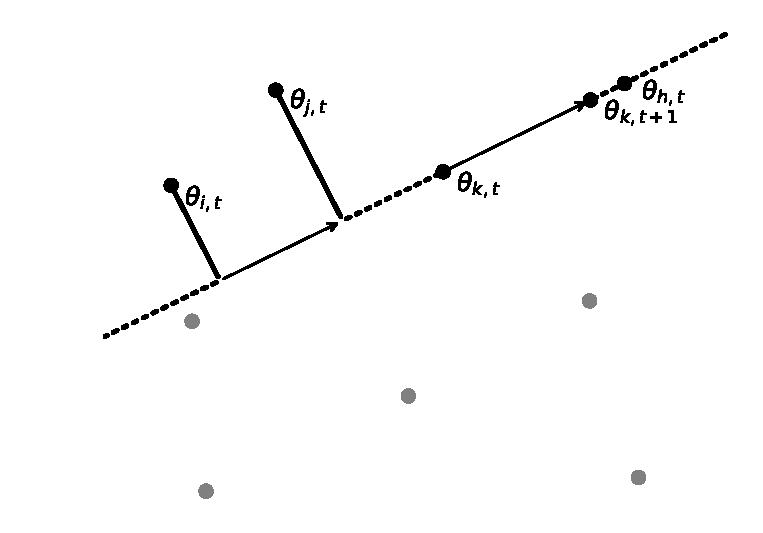
\includegraphics[width=1.0\linewidth]{Figures/snooker_move_2025.eps}
\caption{Snooker update move for chain $k$. A proposal is generated by randomly selecting another chain ($h$) for determining the direction and two chains ($i$ and $j$) for determining the distance. The distance is calculated by projecting $i$ and $j$ orthogonally on the line connecting $k$ to $h$ and subsequently multiplying with a user-defined scalar (here 1.2), resulting in the proposal $\theta_{k,t+1}$.}\label{fig2b}
\end{figure}
\noindent \cite{terbraak2008differential} found that combining Differential Evolution with snooker updates in a 90 to 10 percent ratio leads to the best performance, which is also the setup in this study. They also introduced an algorithm similar to DE-SNK, which requires the use of very few chains (typically 3), by exploiting information from their past by
generating jumps from differences of pairs of past states. Although powerful, sampling from past states was not included as it is not supported by the software used in this study. 

The third and final MCMC algorithm used in this study is the Ensemble Sampler by Goodman and Weare (AI), that utilises the Stretch move (\hyperref[fig1]{\textcolor{blue}{Figure }\ref{fig1}}). \cite{goodman2010ensemble} introduced several affine-invariant MCMC algorithms; hence the name. Here, affine-invariant refers to the algorithm performing well regardless of how skewed the posterior distribution is, e.g. due to strongly correlated parameters. The introduced algorithms utilise different moves, of which the Stretch Move is considered the most powerful \citep{goodman2010ensemble}.

All three samplers are implemented with emcee version 3.1.6 \citep{foreman2013emcee}. Different moves were selected using the \textit{moves} keyword for the (class) \textit{EnsembleSampler}. Since the three samplers only vary in the moves used, selecting different moves results in selecting a different sampler. Optionally, a weighted mixture of moves can be used, as required for DE-SNK. During sampling, at each step, a move is randomly selected from the mixture. For all moves, the default scaling parameters of the emcee package are used, which are consistent with the developers recommendations of said algorithms \citep{terbraak2006markov, terbraak2008differential, goodman2010ensemble}. 

\begin{figure}[ht]
\centering
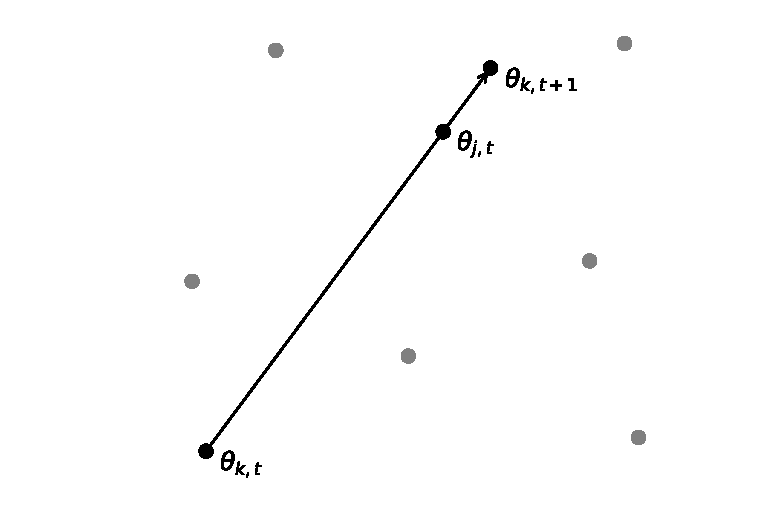
\includegraphics[width=1.0\linewidth]{Figures/stretch_move.eps}
\caption{A stretch move for parameter $\theta$ of chain $k$. The grey dots represent the chains not participating in this move. A proposal is generated by randomly selecting another chain ($j$) and moving in this direction, with the magnitude determined by a user determined scalar (here 1.2), resulting in the proposal $\theta_{k,t+1}$.}\label{fig1}
\end{figure}

\subsection{Performance diagnostics}\label{mcmc eval}
The performance of the different samplers is compared using several diagnostics explained in this section. Chain convergence is evaluated with the Gelman-Rubin diagnostic ($\hat{R}$). Sampling efficiency is assessed with the acceptance rate and the Effective Sample Size (ESS). The posteriors are evaluated on their median, kernel density estimate (KDE) plots and pairs plots. 
%The diagnostics for evaluating the performance of the different samplers are described below. Included are the Integrated Autocorrelation Time, Gelman-Rubin diagnostic, median, acceptance rate, kernel density estimate (KDE) plots and pair plots. % alternatively leave subsection intro empty

\subsubsection{Gelman-Rubin diagnostic}
\cite{gelman1992inference} designed a widely used metric to determine whether one's chains have converged, typically referred to as the Gelman-Rubin diagnostic ($\hat{R}$). This is a ratio between the total variance and the within chain variance (where the total variance is due to both the within and between chain variance).  % can add formulas 13.16 and 13.17 from Students guide to Bayesian statistics.  
As $\hat{R} \to 1$, the chains approach a stationary distribution \citep{lambert2018student}. In practice, when $\hat{R}$ becomes smaller than an arbitrary cutoff value, one's chains are considered to have converged, for which \cite{gelman1992inference} suggested using $\hat{R} \leq 1.1$. 

\cite{gelman2021bayesian} made a small modification to $\hat{R}$, called split-$\hat{R}$, which also compares the first half of each chain to the second half, with the objective to detect lack of convergence within each chain. % \cite{vehtari2021rank} refer to split-R as R, so they consider the 2013 version the new standard...

While very popular, several serious issues have been identified with $\hat{R}$ and split-$\hat{R}$, such as failing to correctly diagnose convergence when the chain has a heavy tail or when the variance varies across the chains. To address these problems, \cite{vehtari2021rank} proposed an alternative rank-based version of $\hat{R}$. In addition \cite{vehtari2021rank} recommends a much more conservative convergence criterion of $\hat{R} \leq 1.01$. 

%Although recommended, 1.01 required impractically long run-times for the hardware used in this study. Therefore, a convergence criterion of 1.05 was used instead. 
The rank-based $\hat{R}$ from \citep{vehtari2021rank} is implemented with the function \textit{rhat} from the \textit{ArviZ} package, version 0.19.0 \citep{kumar2019arviz} and will from now on simply be referred to as $\hat{R}$. 

\subsubsection{Effective Sample Size}
MCMC is a dependent sampling method, resulting in correlation between serial steps of a Markov chain. As a consequence, the effective number of independent samples, called the Effective Sample Size (ESS), is smaller than the total number of steps (\hyperref[eq7a]{\textcolor{blue}{Equation }\ref{eq7a}}).
% definition effective sample size:  how many independent draws contain the same amount of information as the dependent sample obtained by the MCMC algorithm. 
%The correlation between a chain's location and its previous locations is called autocorrelation. The autocorrelation can be computed for different lag values, where lag is the number of steps between the points being compared in the chain. ### This is common knowledge for most hydrologists.
%When the autocorrelation between lagged steps is large and decays slowly, the chain is inefficient and the ESS will be relatively small.

\begin{equation}\label{eq7a}
    \widehat{ESS} = \frac{N}{\hat{\tau}_f}
\end{equation}
Where $N$ represents the total number of steps of the Markov chain and $\hat{\tau}_f$ represents an estimate of the integrated autocorrelation time, which quantifies how many intermediate steps are required for steps to be considered independent. 

For a longer integrated autocorrelation time, more samples must be generated to produce a representative sample of the target density. For a Markov chain $\tau_f$ can theoretically be estimated with \hyperref[eq7]{\textcolor{blue}{Equation} \ref{eq7}}:

\begin{equation}\label{eq7}
    \hat{\tau}_f (N) = 1 + 2 \sum_{\tau=1}^{N} \hat{\rho}_f (\tau) 
\end{equation} 
where $\hat{\tau}_f (N)$ represents an estimate of the integrated autocorrelation time, $N$ represents the number of steps of the Markov chain and $\hat{\rho}_f (\tau)$ represents an estimate of the normalised autocorrelation function. Here, the autocorrelation function is normalised by dividing it by the autocovariance at lag 0.

At larger lags, $\hat{\rho}_f (\tau)$ starts to contain more noise than signal, summing up to N will therefore lead to a noisy estimate of $\hat{\tau}_f$. Instead, \cite{sokal1997monte} recommends estimating $\tau_f$, for some $M \ll N$, with \hyperref[eq8]{\textcolor{blue}{Equation} \ref{eq8}}:  
\begin{equation}\label{eq8}
    \hat{\tau}_f (M) = 1 + 2 \sum_{\tau=1}^{M} \hat{\rho}_f (\tau) 
\end{equation} 
By introducing $M$, the function is evaluated for a smaller number of lags, decreasing the variance at the cost of a small increase in bias.  \cite{sokal1997monte} recommends choosing the smallest value of $M$, where $M \geq C \, \hat{\tau}_f (M)$ and $C \sim 5$. For an extensive discussion on computing the integrated autocorrelation time the reader is referred to %'see' feels informal
\cite{sokal1997monte}, or to \cite{foreman2022autocorr} for a summary of the most important points. %not sure how to cite foreman2022autocorr 
%Sokal says that he finds this procedure to work well for chains longer than, but the situation is a bit better with emcee because we can use the parallel chains to reduce the variance and we’ve found that chains longer than about are often sufficient
Here, $\hat{\tau}_f (M)$ was computed with the function 
\textit{autocorr.integrated\_time}
from the \textit{emcee} package, version 3.1.6 \citep{foreman2013emcee}.

\subsubsection{Other diagnostics}
Generally, groundwater flow models have a constant value for each parameter. On the other hand, MCMC produces an estimated posterior distribution for each parameter. This introduces the challenge of choosing the most suitable value from this distribution to use in the groundwater flow model. Possible options include the distribution mean, median, or mode. The mean has the drawback that it is strongly influenced by extreme values. This is problematic because, the the posterior distributions of the parameters in this study span multiple orders of magnitude. Selecting the mode of the distribution may be an intuitive value to use in the groundwater flow model. However, problems arise when the distribution is multimodal (the tallest mode, may e.g. have little width, making it challenging to select a mode). Since the median does not have the drawbacks of the mean and mode, it has been selected as the point estimator to use for parameters in MODFLOW 6. %In this study the ensemble median has been selected for this purpose. % specify that the median was implemented with scripts developed by the author?

The fraction of proposed steps that are accepted is called the acceptance rate, giving an indication of sampling efficiency. If the acceptance rate approaches 1, most proposals are accepted, resulting in inefficient random-walk behaviour. An acceptance rate close to 0 on the other hand, results in inefficiency due to the chain being mostly stuck in the same place. 

\cite{gelman1997weak} found that optimal acceptance rates for the Metropolis algorithm scale with dimensionality (number of calibrated parameters), starting at about 0.44 for 1 dimension and decreasing to about 0.23 for highly dimensional problems. The optimal acceptance rate decreases with dimensionality because, for higher dimensional problems, the 'volume' containing posterior density becomes increasingly small relative to the remainder of parameter space \citep{mackay2003information}. Although the optimal acceptance rates found by \cite{gelman1997weak} are for the Metropolis algorithm, the results are widely used as a guideline for other samplers, including by \cite{terbraak2006markov} for DE. More recently \cite{schmon2022optimal} found optimal Metropolis acceptance rates for specific dimensional problems. By adjusting the tuning parameters of a sampler (e.g. the width of the proposal distribution for Metropolis), different acceptance rates can be achieved. However, for Ensemble Samplers, default tuning parameters are typically used (also in this study, see \hyperref[mcmc used]{\textcolor{blue}{Section }\ref{mcmc used}}). Therefore, considering sampling efficiency, it is useful to examine whether default tuning parameters for the samplers used in this study result in (close to) optimal acceptance rates. %No existing Python packages were used to compute the acceptance rates, but scripts developed by the author. OR leave it out because by not mentioning I imply that I wrote these scripts?

Kernel density estimate (KDE) plots represent the posterior samples using a continuous probability density curve, providing a clear visualization of the posterior distributions of each parameter. KDE plots were used for identifying multimodality and for comparing the posteriors produced by different samplers. %and scenarios
KDE plots were implemented using the function \textit{kdeplot} from the \textit{Seaborn} package, version 0.13.2 \citep{Waskom2021}.

A pairs plot is a matrix of graphs that visualizes the relationship between parameters by pairwise comparison. It combines both histogram and scatter plots, providing an overview of estimated posterior distributions and parameter covariance. Pairs plots were implemented (with a KDE style) using the function \textit{pairplot} from the \textit{Seaborn} package. % repeat version or not? 

\subsection{Synthetic scenarios}\label{mcmc exp}
The MCMC samplers (DE, DE-SNK and AI) are compared in a calibration exercise. Four simple steady-state synthetic groundwater flow models (designed using MODFLOW 6) were calibrated, which are described in \hyperref[gfm]{\textcolor{blue}{Section }\ref{gfm}}. The performance of the samplers is evaluated in different scenarios, in which not only different models are used, but also different priors and number of observations, as described in \hyperref[mcmc setup]{\textcolor{blue}{Section }\ref{mcmc setup}}.

\subsubsection{Groundwater flow models}\label{gfm}
The four synthetic groundwater flow models designed for this study are shown in \hyperref[fig_sgm]{\textcolor{blue}{Figure }\ref{fig_sgm}}. These models were developed using MODFLOW 6, version 6.5.0 \citep{langevin2017modflow}. To create, run and post-process these models, FloPy version 3.8.1 was used \citep{hughes2023flopy}. The parameters $inner\_maximum$ and $outer\_maximum$ from FloPy's Iterative Model Solution package were both increased from their default values (25 and 50, respectively) to 1000, allowing more iterations for the solver. This solved MODFLOW simulation errors encountered during testing runs (\hyperref[sim_error]{\textcolor{blue}{Appendix }\ref{sim_error}}). 

The hydraulic conductivities presented in \hyperref[fig_sgm]{\textcolor{blue}{Figure }\ref{fig_sgm}} represent the 'true' values for each model. Running each model with these 'true' hydraulic conductivities results in the 'true' hydraulic heads for every model cell. With the well located in the phreatic layer in every model, one would expect flow paths to be towards the well for all layers. This is indeed the case as can be seen by the deeper layers having increasingly large hydraulic heads (\hyperref[fig_heads_side]{\textcolor{blue}{Figure }\ref{fig_heads_side}}).

To simulate the effects of measurement errors of hydraulic head measurements performed in the field, noise was added to the ’true’ hydraulic heads of every model cell. \cite{rau2019error} compared eight different electric dip meters and found that the random measurement error varied by several centimeters depending on the operator and the water depth. Furthermore, it was

\begin{figure}[ht]
\centering
\includegraphics[width=1.0\linewidth]{Figures/CONGROMO_NEW4.JPG}
\caption{Schematic of the four steady-state synthetic groundwater flow models used in this study. Layer thickness ($z_n$) and the respective isotropic hydraulic conductivities ($\theta_n$) are shown inside each layer ($n$). The models have a length and width of 1000 meters, consisting of 25 rows and columns with a length of 40 meters. The total depth of each model equals 50 meters. At the centre of each model is an abstraction well (indicated by the building) with an extraction rate of 500 m\textsuperscript{3}/day. The well screens extend over the full depth of the phreatic aquifer of the respective model, resulting in e.g. a 50 meter long well screen for Model 1, versus a 15 meter long well screen for Model 4. At the model edges, there are constant head boundaries of 10 meters.}\label{fig_sgm} %so the location of the label influences how it is referenced!?, that's clunky
\end{figure} %Above each model, its name is given with the number of calibrated parameters indicated by the subscript.

\begin{figure}[htb!]
\centering
\includegraphics[width=1.0\linewidth]{Figures/heads_side.png}
\caption{Side view of the true hydraulic heads (m) in all models. The side view shows row 12 out of 25 rows total, indexing from 0. The x axis shows the columns of the different models (also 25 total). Note that layer 1 always refers to the uppermost layer, with deeper layers having sequentially greater numbers.\label{fig_heads_side}}
\end{figure} % fix widt back to 1 possibly as it looks nicer

\noindent shown by \cite{rau2019error} that the magnitude of systematic errors tends to be much larger than that 

\begin{table*}[htb]
\caption{Priors for the hydraulic conductivities in the designed groundwater flow models. The presented prior distributions (truncated normal) are transformed for use by the MCMC samplers\textsuperscript{[1]}. For each prior, a formula is presented to transform the respective parameter as used in MCMC ($\theta_{\text{mc}}$), to a hydraulic conductivity in m/d ($\theta_{\text{mod}}$). For the narrow prior, $\mathcal{O}$ is introduced, which represents log10() of the 'true' hydraulic conductivity (m/d), subsequently rounded down to an integer (in python: math.floor(math.log10(x))).}
\label{tab_priors}
\setlength{\tabcolsep}{13pt} %can manually adjust column spacing
\begin{tabularx}{\textwidth}{lllll}
\toprule
Name & Sediment & Prior distribution & Transformation (m/d) & bounds (m/d) \\
\midrule
Wide & clean sand & $\mathcal{TN}(0, 0.5^2, -1, 1)$ & $\theta_{\text{mod}} = 10^{2\theta_{\text{mc}} + 1}$ & [$10^{-1},10^3]$\\
Wide & silty sand  & $\mathcal{TN}(0, 0.5^2, -1, 1)$ & $\theta_{\text{mod}} = 10^{2\theta_{\text{mc}}}$ &  [$10^{-2},10^2]$\\
Wide & silt, loess   & $\mathcal{TN}(0, 0.5^2, -1, 1)$  & $\theta_{\text{mod}} = 10^{2\theta_{\text{mc}} - 1}$  & [$10^{-3},10^1]$\\
\midrule
Narrow & - & $\mathcal{TN}(0, 0.125^2, -1, 1)$  &  $\theta_{\text{mod}} = 10^{2\theta_{\text{mc}} + \mathcal{O}}$ & [$10^{-2+\mathcal{O}},10^{2+\mathcal{O}}]$\\
\bottomrule
\end{tabularx}
\end{table*}

\noindent of random errors. Systematic errors can have a constant bias (e.g. poorly calibrated equipment) or a non-constant bias (e.g. salinity can result in a linearly increasing bias with depth due to density differences compared to fresh water). %, similarly a borehole drilled under an angle can result in linearly increasing bias with depth). 
For simplicity, all errors were lumped into a Gaussian distribution with an inflated variance based on these findings. Measurement noise was added $\epsilon \sim N(0,0.1)$, with the mean and standard deviation in meters.

After adding noise to all hydraulic heads, observation locations were selected stochastically. This was achieved by randomly generating numbers between 2 and 24 using the function \textit{randint} from Python's built-in \textit{random} module, with each number specifying the row or column of a cell in the model. Cells on the boundary of the model, with corresponding row and column integers of 1 and 25, are excluded from being selected as measurement locations, due to the boundary conditions at the edges of the models. If by chance the same x,y coordinates are selected more than once, resampling occurs. If the model has multiple layers, selected observations are always on top of each other, similar to how one measurement well contains multiple piezometers in different layers. 

To provide insight into the importance of the amount of available data, three scenarios per model were created. The scenarios differ in the number of observations per layer: 1, 3 or 5. For a more complex model this results in a greater number of total observations than a simpler model, but in the same amount of observations per layer (i.e. per parameter). 

\subsubsection{MCMC setup}\label{mcmc setup}
Six different prior-likelihood combinations (scenarios) were created for each of the four synthetic groundwater flow models shown in \hyperref[fig_sgm]{\textcolor{blue}{Figure }\ref{fig_sgm}}. These scenarios differ in: prior knowledge (on hydraulic conductivities) and available data (number of hydraulic head measurements for computing the likelihood). 

The priors are similar to what may be used in a real case study, by using representative values of the respective sediments/geological materials. For each layer of each model two different priors were created, from now on referred to as the narrow and wide prior. 

The wide priors are based on lithology (supposedly) found in the respective layers during e.g. piezometer construction. The prior bounds for hydraulic conductivities are inspired by the ranges for clean sand, silty sand, and silt presented in \cite{woessner2020hydrogeologic}. The 'true' hydraulic conductivity value of each layer was designed to fall within the prior bounds of the lithology found within each layer (see \hyperref[tab_priors]{\textcolor{blue}{Table }\ref{tab_priors}} for the priors and \hyperref[tab_priors_lithology]{\textcolor{blue}{Appendix }\ref{tab_priors_lithology}} for the lithology of each layer). 

\begin{figure}[htb]
\centering
\includegraphics[width=1.0\linewidth]{Figures/priors.png}
\caption{Prior distributions for the hydraulic conductivity of layer 1 in Model 2 (contains clean sand), with \textbf{A)} showing the wide prior and \textbf{B)} the narrow prior. The top x-axes indicate the parameter values used by the MCMC algorithm, while the bottom x-axes show the corresponding transformed hydraulic conductivity values (m/d) as used by MODFLOW 6. The priors are truncated at the plot boundaries. The dotted red line indicates the true hydraulic conductivity.}\label{fig_priors}
\end{figure} 

\footnotetext[1]{The applied parameter transformations differ from statistical convention. Conventionally, the transformation for the likelihood function would simply take the exponent of the parameter: $\theta_{mod} = 10^{\theta_{mc}}$. The prior for e.g. clean sand would then be $\mathcal{TN}(1, 1, -1, 3)$ and the prior for silty sand would be $\mathcal{TN}(0, 1, -2, 2)$. However, the result of both methods on inference is the same.}% can replace methods with approaches

For the narrow prior, it is assumed that a much more precise estimate of the hydraulic conductivity of each layer is available (e.g. from pumping tests). The narrow priors have a standard deviation four times smaller than that of the wide priors. Additionally, the centre of the narrow prior distribution depends on the 'true' hydraulic conductivity (\hyperref[tab_priors]{\textcolor{blue}{Table }\ref{tab_priors}}). Note that the centre of the narrow prior is within an order of magnitude distance from the 'true' hydraulic conductivity (\hyperref[tab_priors]{\textcolor{blue}{Table }\ref{tab_priors}}). An example of the narrow and wide prior distributions is shown in \hyperref[fig_priors]{\textcolor{blue}{Figure }\ref{fig_priors}}. 

With hydraulic conductivities spanning many orders of magnitude, numerical stability of the MCMC samplers was a concern. Parameter transformation was applied to address this issue. The parameters were transformed at each step of the Markov chain, to a hydraulic conductivity in meters per day (\hyperref[tab_priors]{\textcolor{blue}{Table }\ref{tab_priors}}). 
Subsequently, the respective model was run in MODFLOW 6 with the transformed parameters. For each selected observation location, the difference was calculated between the hydraulic heads produced by this model run and the noisy observations ($\delta h$). For each observation, $\delta h$ was inserted into the log probability density function (logpdf) of the error. The log-likelihood was computed as the sum of the logpdf of every observation. The selected likelihood distribution is $\mathcal{N}(0,0.1)$, which is identical to the distribution that was used to generate the measurement noise. % is this a correct likelihood?
Priors and likelihood were implemented with the functions \textit{truncnorm}, \textit{norm} and \textit{logpdf} from the \textit{SciPy.stats} package, version 1.11.4 \citep{2020SciPy-NMeth}. % or module?
% no Jacobian adjustment was necesarry because: the difference between a change of variables and a simple variable transformation. A transformation samples a parameter, then transforms it, whereas a change of variables transforms a parameter, then samples it. Only the latter requires a Jacobian adjustment. https://mc-stan.org/docs/stan-users-guide/reparameterization.html#changes-of-variables

Chain initialisation was performed by taking a random sample from the respective prior distribution with the \textit{rvs} function from the \textit{SciPy.stats} package. This was programmed with a constant seed, to ensure that identical datasets were used for chain initialisation of different samplers and scenarios.

For each of the six scenarios (prior-likelihood combinations), five ensembles were run per sampler (AI, DE and DE-SNK), each consisting of 10 chains with a length of 2000 steps. This procedure was carried out for all (four) designed synthetic groundwater flow models. Trace plots of testing runs showed good mixing of the Markov chains within 1000 steps. Therefore, burn-in was set at 1000 steps, leaving 1000 steps per chain for estimation of the posterior distribution. 

\newpage

\FloatBarrier

\section{Results}\label{results}
This chapter presents the results of calibrating Model 1-4 with the MCMC samplers: AI, DE and DE-SNK, for the scenarios described above. The efficiency of the samplers is evaluated using acceptance rates and the estimated Effective Sample Size ($\widehat{ESS}$). Subsequently, chain convergence is assessed with the Gelman-Rubin diagnostic ($\hat{R}$). 
Next, samplers are compared based on how closely their posterior medians approximate the true hydraulic conductivities. 
Finally, the shape of the posterior distributions and the relationship between different parameters is investigated with Kernel Density Estimate plots (KDE) and pairs plots, respectively.   

The acceptance rate of proposed steps varies strongly between the different samplers, with the Affine-Invariant sampler (AI) reporting the highest acceptance rates (\hyperref[tab_fracs]{\textcolor{blue}{Table }\ref{tab_fracs}}). The observed acceptance rate for all samplers decreases when the number of calibrated parameters increases, considering that dimensionalities for Model 1 up to Model 4 are 1,2,3 and 5, respectively. 
The optimal acceptance rate according to theory is 0.44 for 1 dimension, decreasing to 0.28 for 5 dimensions and asymptotically approaching 0.23 for even higher dimensions \citep{schmon2022optimal, terbraak2006markov}. For DE-based strategies, most acceptance rates closely align with these optimal values. Except for too low values when using the wide prior for Model 3 and 4. In contrast, AI reports too high acceptance rates for most scenarios. Regarding prior choice, using the narrow prior resulted on average in more optimal acceptance rates for DE and DE-SNK, but not for AI. % caused by initialisation far true posterior density? OR due to prior shifted away from true posterior density? 
The variability in acceptance rates between chains of a specific sampler for a specific scenario is relatively small, indicated by the compactness of the boxplots, suggesting consistency between different ensembles (\hyperref[tab_fracs]{\textcolor{blue}{Table }\ref{tab_fracs}}).

\begin{table*}[ht]
\centering
\caption{Acceptance rates for each scenario are presented with boxplots. Each boxplot was constructed using acceptance rates of the last 1000 steps of 50 chains (5 ensembles of 10 chains). Optimal Metropolis acceptance rates, based on dimensionality, are indicated with dashed red lines: 0.44 for Model 1, 0.35 for Model 2, 0.31 for Model 3 and 0.28 for Model 4 \citep{schmon2022optimal}. Although invisible, all boxplots in the same column share the same x-axis and thus can be compared. Additionally, average row acceptance rates are provided in the rightmost column and average column acceptance rates are provided in the bottom row.}
\label{tab_fracs}
\begin{tabularx}{\textwidth}{llXXXXXXl}
\toprule
\multirow{2}{*}{Model} & \multirow{2}{*}{Sampler} & \multicolumn{3}{c}{Wide prior} & \multicolumn{3}{c}{Narrow prior} & \multirow{2}{*}{Average}\\
\cmidrule(lr){3-5} \cmidrule(lr){6-8}
& & \multicolumn{1}{c}{1 obs} & \multicolumn{1}{c}{3 obs} & \multicolumn{1}{c}{5 obs} & \multicolumn{1}{c}{1 obs} & \multicolumn{1}{c}{3 obs} & \multicolumn{1}{c}{5 obs} & \\
\cmidrule(lr){1-2} \cmidrule(lr){3-5} \cmidrule(lr){6-8} \cmidrule(lr){9-9}
\multirow{3}{*}{1} & AI & \multicolumn{3}{c}{\multirow{3}{*}{\includegraphics[width=6cm]{Figures/boxplots_model1_priorbroad.png}}} & \multicolumn{3}{c}{\multirow{3}{*}{\includegraphics[width=6cm]{Figures/boxplots_model1_priornarrow.png}}} & \textbf{0.73}\\
& DE & \multicolumn{3}{c}{} & \multicolumn{3}{c}{} & \textbf{0.40}\\
& DE-SNK & \multicolumn{3}{c}{} & \multicolumn{3}{c}{} & \textbf{0.44}\\
\cmidrule(lr){1-2} \cmidrule(lr){3-5} \cmidrule(lr){6-8} \cmidrule(lr){9-9}
\multirow{3}{*}{2} & AI & \multicolumn{3}{c}{\multirow{3}{*}{\includegraphics[width=6cm]{Figures/boxplots_model2_priorbroad.png}}} & \multicolumn{3}{c}{\multirow{3}{*}{\includegraphics[width=6cm]{Figures/boxplots_model2_priornarrow.png}}} & \textbf{0.64}\\
& DE & \multicolumn{3}{c}{} & \multicolumn{3}{c}{} & \textbf{0.28}\\
& DE-SNK & \multicolumn{3}{c}{} & \multicolumn{3}{c}{} & \textbf{0.33}\\
\cmidrule(lr){1-2} \cmidrule(lr){3-5} \cmidrule(lr){6-8} \cmidrule(lr){9-9}
\multirow{3}{*}{3} & AI & \multicolumn{3}{c}{\multirow{3}{*}{\includegraphics[width=6cm]{Figures/boxplots_model3_priorbroad.png}}} & \multicolumn{3}{c}{\multirow{3}{*}{\includegraphics[width=6cm]{Figures/boxplots_model3_priornarrow.png}}} & \textbf{0.56}\\
& DE & \multicolumn{3}{c}{} & \multicolumn{3}{c}{} & \textbf{0.24}\\
& DE-SNK & \multicolumn{3}{c}{} & \multicolumn{3}{c}{} & \textbf{0.30}\\
\cmidrule(lr){1-2} \cmidrule(lr){3-5} \cmidrule(lr){6-8} \cmidrule(lr){9-9}
\multirow{3}{*}{4} & AI & \multicolumn{3}{c}{\multirow{3}{*}{\includegraphics[width=6cm]{Figures/boxplots_model4_priorbroad.png}}} & \multicolumn{3}{c}{\multirow{3}{*}{\includegraphics[width=6cm]{Figures/boxplots_model4_priornarrow.png}}} & \textbf{0.44}\\
& DE & \multicolumn{3}{c}{} & \multicolumn{3}{c}{} & \textbf{0.16}\\
& DE-SNK & \multicolumn{3}{c}{} & \multicolumn{3}{c}{} & \textbf{0.25}\\
\midrule
\multicolumn{2}{l}{\textbf{Average}} & \hspace{13pt}\textbf{0.37} & \hspace{13pt}\textbf{0.30} & \hspace{13pt}\textbf{0.38} & \hspace{13pt}\textbf{0.46} & \hspace{13pt}\textbf{0.43} & \hspace{13pt}\textbf{0.43} & \textbf{-}\\
\bottomrule
\end{tabularx}
\end{table*}

\begin{table*}[hbt]
\centering
\caption{The Estimated Effective Sample Size ($\widehat{ESS}$) for each scenario. The presented values were obtained by first calculating the mean $\widehat{ESS}$ for the last 1000 steps of each chain. Then, the sum was taken for all 10 chains of all 5 ensembles (50 chains total and 50,000 samples). For interpretability, row and column averages are also provided.}
\label{tab_ess_mean}
\begin{tabularx}{\textwidth}{llXXXXXXX}
\toprule
\multirow{2}{*}{Model} & \multirow{2}{*}{Sampler} & \multicolumn{3}{c}{Wide prior} & \multicolumn{3}{c}{Narrow prior} & \multirow{2}{*}{Average}\\
\cmidrule(lr){3-5} \cmidrule(lr){6-8} 
& & 1 obs & 3 obs & 5 obs & 1 obs & 3 obs & 5 obs & \\
\cmidrule(lr){1-2} \cmidrule(lr){3-5} \cmidrule(lr){6-8} \cmidrule(lr){9-9}
\multirow{3}{*}{1} & AI & 2462 & 2291 & 2422 & 3341 & 2878 & 3036 &  \textbf{2738} \\
& DE & 9377 & 5755 & 9241 & 7743 & 10708 & 5165 & \textbf{7998} \\
& DE-SNK & 8534 & 4637 & 8902 & 7460 & 9193 & 5212 & \textbf{7323}\\
\cmidrule(lr){1-2} \cmidrule(lr){3-5} \cmidrule(lr){6-8} \cmidrule(lr){9-9}
\multirow{3}{*}{2} & AI & 2867 & 1686 & 3009 & 4252 & 3506 & 4210 & \textbf{1567}\\
& DE & 3498 & 1801 & 4147 & 6241 & 4459 & 6508 & \textbf{4442}\\
& DE-SNK & 3840 & 1906 & 4045 & 6168 & 4278 & 5953 & \textbf{4365}\\
\cmidrule(lr){1-2} \cmidrule(lr){3-5} \cmidrule(lr){6-8} \cmidrule(lr){9-9}
\multirow{3}{*}{3} & AI & 1065 & 903 & 1276 & 1673 & 1612 & 1851 & \textbf{1397}\\
& DE & 2323 & 1629 & 2494 & 4787 & 4131 & 4393 & \textbf{3293} \\
& DE-SNK & 2585 & 1620 & 2890 & 4383 & 3706 & 4292 & \textbf{3246} \\
\cmidrule(lr){1-2} \cmidrule(lr){3-5} \cmidrule(lr){6-8} \cmidrule(lr){9-9}
\multirow{3}{*}{4} & AI & 807 & 670 & 805 & 1202 & 1094 & 1075 & \textbf{942}\\
& DE & 1333 & 851 & 1026 & 2719 & 2045 & 2063 & \textbf{1673}\\
& DE-SNK & 1514 & 921 & 1462 & 2748 & 2369 & 2326 & \textbf{1890}\\
\midrule
\textbf{Average} &  & \textbf{3228} & \textbf{1985} & \textbf{3345} & \textbf{4207} & \textbf{4015} & \textbf{3657} & - \\
\bottomrule
\end{tabularx}
\end{table*}

The estimated Effective Sample Size ($\widehat{ESS}$) decreases with increasing model number (\hyperref[tab_ess_mean]{\textcolor{blue}{Table }\ref{tab_ess_mean}}). This is what was expected based on the acceptance rate also decreasing with increasing Model number (\hyperref[tab_fracs]{\textcolor{blue}{Table }\ref{tab_fracs}}). Although AI has the highest acceptance rate, its $\widehat{ESS}$ is actually the lowest for almost all scenarios. Thus, the autocorrelation of Markov chains must be relatively high for AI, implying that the AI 'Stretch' move produces relatively poor proposals. There is no clear 

\newpage
\noindent winner for $\widehat{ESS}$, with DE and DE-SNK reporting similar values for most models, except for Model 4, for which DE-SNK consistently outperforms DE. Using more observations for likelihood evaluations appears to have a negative effect on the $\widehat{ESS}$, although not distinctly (column totals \hyperref[tab_ess_mean]{\textcolor{blue}{Table }\ref{tab_ess_mean}}). Using a more informative prior does appear to have a positive effect on the $\widehat{ESS}$ (\hyperref[tab_ess_mean]{\textcolor{blue}{Table }\ref{tab_ess_mean}}), consistent with more optimal acceptance rates for the narrow prior (\hyperref[tab_fracs]{\textcolor{blue}{Table }\ref{tab_fracs}}). % consider adding a comment about the variation between different ensembles (standard deviation presented as percentage may atleast for my analysis be valuable

\begin{table*}[ht]
\centering
\caption{The number of ensembles with all Gelman-Rubin diagnostic values ($\hat{R}$) below the threshold of 1.05. First, $\hat{R}$ was calculated for all parameters using the last 1000 steps of each chain per ensemble. Then, the ensembles with all $\hat{R} < 1.05$ were counted for each scenario. For interpretability, row and column averages are also provided.}
\label{tab_rhat_mean}
\begin{tabularx}{\textwidth}{llXXXXXXX}
\toprule
\multirow{2}{*}{Model} & \multirow{2}{*}{Move} & \multicolumn{3}{c}{Wide prior} & \multicolumn{3}{c}{Narrow prior} & \multirow{2}{*}{Average}\\
\cmidrule(lr){3-5} \cmidrule(lr){6-8}
& & 1 obs & 3 obs & 5 obs & 1 obs & 3 obs & 5 obs & \\
\midrule
\multirow{3}{*}{1} & AI & 5 & 5 & 4 & 2 & 1 & 1 & \textbf{3.00} \\
& DE & 5 & 5 & 5 & 5 & 5 & 0 & \textbf{4.17} \\
& DE-SNK & 5 & 5 & 5 & 5 & 2 & 0 & \textbf{3.67} \\
\cmidrule(lr){1-2} \cmidrule(lr){3-5} \cmidrule(lr){6-8} \cmidrule(lr){9-9}
\multirow{3}{*}{2} & AI & 0 & 0 & 1 & 4 & 2 & 2 & \textbf{1.50} \\
& DE & 5 & 4 & 5 & 5 & 5 & 5 & \textbf{4.83} \\
& DE-SNK & 5 & 3 & 5 & 5 & 5 & 5 & \textbf{4.67} \\
\cmidrule(lr){1-2} \cmidrule(lr){3-5} \cmidrule(lr){6-8} \cmidrule(lr){9-9}
\multirow{3}{*}{3} & AI & 0 & 0 & 0 & 2 & 0 & 3 & \textbf{0.83} \\
& DE & 4 & 1 & 4 & 5 & 5 & 5 & \textbf{4.00} \\
& DE-SNK 3 & 5 & 0 & 4 & 5 & 5 & 5 & \textbf{4.00} \\
\cmidrule(lr){1-2} \cmidrule(lr){3-5} \cmidrule(lr){6-8} \cmidrule(lr){9-9}
\multirow{3}{*}{4} & AI & 0 & 0 & 0 & 0 & 0 & 0 & \textbf{0.00} \\
& DE & 0 & 0 & 0 & 5 & 1 & 4 & \textbf{1.67} \\
& DE-SNK & 1 & 0 & 0 & 5 & 5 & 4 & \textbf{2.50} \\
\midrule
\textbf{Average} & & \textbf{2.92} & \textbf{1.92} & \textbf{2.75} & \textbf{4.00} & \textbf{3.00} & \textbf{2.83} & \textbf{-} \\
\bottomrule
\end{tabularx}
\end{table*}

Too few ensembles passed the recommended $\hat{R}$ threshold of 1.01 by \cite{vehtari2021rank} for any meaningful comparison. Therefore, the threshold in \hyperref[tab_rhat_mean]{\textcolor{blue}{Table }\ref{tab_rhat_mean}} was relaxed to 1.05, which is still relatively strict compared to the original recommendation of 1.10 by \cite{gelman1992inference}. AI reports the fewest ensembles with all $\hat{R}$ below the threshold of 1.05 for each model, suggesting that AI convergences relatively poorly (\hyperref[tab_rhat_mean]{\textcolor{blue}{Table }\ref{tab_rhat_mean}}). This aligns with AI reporting the lowest $\widehat{ESS}$ values, as chains tend to have a longer integrated autocorrelation time ($\tau_f$) during burn-in \citep{hogg2018data}. Using the narrow prior results in more ensembles with all $\hat{R}$ below the threshold for Model 2,3 and 4, indicating improved convergence. This trend is consistent with $\widehat{ESS}$ being larger for Model 2,3 and 4, when using the narrow prior (\hyperref[tab_ess_mean]{\textcolor{blue}{Table }\ref{tab_ess_mean}}). For models with more parameters (higher model number), $\hat{R}$ indicates worse convergence for all samplers (\hyperref[tab_rhat_mean]{\textcolor{blue}{Table }\ref{tab_rhat_mean}}).

The median parameter values of all steps of all chains of all (5) ensembles for a scenario (from now on referred to as simply the median), are extremely similar for the different samplers  (\hyperref[tab_median_color]{\textcolor{blue}{Table }\ref{tab_median_color}}), even though AI showed the worst acceptance rate, $\widehat{ESS}$ and $\hat{R}$. The median is a much better estimate of the true parameter values ($\theta_{n,\,true}$) when using the narrow prior, opposed to using the wide prior. This difference is especially striking for parameters with a low $\theta_{n,\,true}$. Increasing the number of observations for evaluating the likelihood clearly improves the estimate of $\theta_{n,\,true}$, which is again most striking for parameters with a low $\theta_{n,\,true}$. Interestingly, using more observations was shown to decrease convergence, yet the estimate of $\theta_{n,\,true}$ improves. This suggests that using more observations leads to a better estimate of the true posterior at the cost of a longer burn-in time. 

The influence of the prior on the shape of the posterior appears strong, with the wide prior resulting in a much broader posterior (\hyperref[fig_kde_model1_DEsnooker]{\textcolor{blue}{Figure }\ref{fig_kde_model1_DEsnooker}}). These Kernel Density Estimate (KDE) plots also reveal a second mode for $\theta_1$ of Model 1, though it contains comparatively little density. Interestingly, the second optimum is (visually) absent for the scenario, where the wide prior is used in combination with three observations for evaluating the likelihood.  \hyperref[fig_kde_model1_DEsnooker]{\textcolor{blue}{Figure }\ref{fig_kde_model1_DEsnooker}} only shows results for DE-SNK, but plots for AI and DE reveal very similar posteriors (appendix figures \ref{fig_kde_model1_Stretch} and \ref{fig_kde_model1_DE}), which is consistent with \hyperref[tab_median_color]{\textcolor{blue}{Table }\ref{tab_median_color}} showing little variation of the Median from different samplers.  

Pairs plots were created for Model 2-4 to identify the posterior distributions and parameter covariances. For conciseness, pairs plots are limited to the scenario with the wide prior and 1 observation per layer. Additionally, only pairs plots for DE-SNK are shown, as different samplers produced similar pairs plots (\hyperref[additional_results]{\textcolor{blue}{Appendix }\ref{sub_pairsplots}}).  

For Model 2, both parameters show a strongly skewed unimodal distribution (\hyperref[fig_kde_model2_DEsnooker]{\textcolor{blue}{Figure }\ref{fig_kde_model2_DEsnooker}}), with the posterior of the upper layer, $\text{p}(\theta_1 | \text{data})$, being much narrower than $\text{p}(\theta_2 | \text{data})$. The joint distribution reveals that $\theta_1$ is largely insensitive to $\theta_2$, if $\theta_2 \lessapprox 0$.  

\begin{table*}[ht]
\centering
\caption{Median parameter values of all (5) ensembles, with $\theta_n$ representing the hydraulic conductivity (m/d) of layer $n$. The true hydraulic conductivities are given between parentheses in column two (Parameter). Each coloured cell represents a scenario (for which 5 ensembles were run), described by the row and column labels. The colour of each cell is an indication of how much the cell value differs from the true hydraulic conductivity of the respective layer (absolute log difference), with dark green representing no difference (best) and red representing large differences (worst). The absolute log difference was used to determine cell colours, because different parameters are of different orders of magnitude.}
\label{tab_median_color}
\begin{tabularx}{\textwidth}{lllXXXXXX}
\toprule
\multirow{2}{*}{Model} & \multirow{2}{*}{Parameter} & \multirow{2}{*}{Move} & \multicolumn{3}{c}{Wide prior} & \multicolumn{3}{c}{Narrow prior} \\
\cmidrule(lr){4-6} \cmidrule(lr){7-9}
& & & 1 obs & 3 obs & 5 obs & 1 obs & 3 obs & 5 obs \\
\midrule
\multirow{3}{*}{1} & \multirow{3}{*}{$\theta_1 \:\: (5.0)$} & AI & 13 \cellcolor[HTML]{C8E300} & 4.1 \cellcolor[HTML]{289300} & 19 \cellcolor[HTML]{FFE400} & 2.2 \cellcolor[HTML]{A8D300} & 2.7 \cellcolor[HTML]{80BF00} & 3.1 \cellcolor[HTML]{61B000} \\
& & DE & 12 \cellcolor[HTML]{C0DF00} & 4.1 \cellcolor[HTML]{2A9400} & 20 \cellcolor[HTML]{FFD800} & 2.3 \cellcolor[HTML]{A6D200} & 2.8 \cellcolor[HTML]{79BC00} & 3.0 \cellcolor[HTML]{68B300} \\
& & DE-SNK & 12 \cellcolor[HTML]{BCDD00} & 4.0 \cellcolor[HTML]{2C9500} & 19 \cellcolor[HTML]{FFE800} & 2.2 \cellcolor[HTML]{A8D300} & 2.7 \cellcolor[HTML]{7EBE00} & 3.1 \cellcolor[HTML]{64B100} \\
\cmidrule(lr){1-3} \cmidrule(lr){4-6} \cmidrule(lr){7-9}
\multirow{6}{*}{2} & \multirow{3}{*}{$\theta_1 \:\: (2.0)$} & AI & 1.9 \cellcolor[HTML]{0A8400} & 1.9 \cellcolor[HTML]{0E8600} & 2.9 \cellcolor[HTML]{49A400} & 1.3 \cellcolor[HTML]{54A900} & 1.4 \cellcolor[HTML]{41A000} & 1.9 \cellcolor[HTML]{068200} \\
& & DE & 2.0 \cellcolor[HTML]{008000} & 2.0 \cellcolor[HTML]{008000} & 2.9 \cellcolor[HTML]{4CA500} & 1.4 \cellcolor[HTML]{4EA600} & 1.4 \cellcolor[HTML]{46A200} & 1.9 \cellcolor[HTML]{068200} \\
& & DE-SNK & 2.0 \cellcolor[HTML]{008000} & 1.9 \cellcolor[HTML]{088300} & 2.9 \cellcolor[HTML]{4CA500} & 1.3 \cellcolor[HTML]{51A800} & 1.4 \cellcolor[HTML]{44A100} & 1.9 \cellcolor[HTML]{088300} \\
\cmidrule(lr){4-6} \cmidrule(lr){7-9}
& \multirow{3}{*}{$\theta_2 \:\: (1.0)$} & AI & 0.92 \cellcolor[HTML]{108700} & 1.0 \cellcolor[HTML]{008000} & 0.46 \cellcolor[HTML]{A2D000} & 1.3 \cellcolor[HTML]{3A9C00} & 1.4 \cellcolor[HTML]{49A400} & 1.4 \cellcolor[HTML]{409F00} \\
& & DE & 0.83 \cellcolor[HTML]{269200} & 0.86 \cellcolor[HTML]{208F00} & 0.54 \cellcolor[HTML]{80BF00} & 1.3 \cellcolor[HTML]{3A9C00} & 1.4 \cellcolor[HTML]{4CA500} & 1.4 \cellcolor[HTML]{46A200} \\
& & DE-SNK & 0.79 \cellcolor[HTML]{309700} & 0.96 \cellcolor[HTML]{088300} & 0.57 \cellcolor[HTML]{76BA00} & 1.3 \cellcolor[HTML]{3A9C00} & 1.4 \cellcolor[HTML]{49A400} & 1.4 \cellcolor[HTML]{48A300} \\
\cmidrule(lr){1-3} \cmidrule(lr){4-6} \cmidrule(lr){7-9}
\multirow{9}{*}{3} & \multirow{3}{*}{$\theta_1 \:\: (1.0)$} & AI & 0.90 \cellcolor[HTML]{148900} & 0.89 \cellcolor[HTML]{188B00} & 1.3 \cellcolor[HTML]{309700} & 1.1 \cellcolor[HTML]{168A00} & 0.89 \cellcolor[HTML]{168A00} & 1.2 \cellcolor[HTML]{229000} \\
& & DE & 0.83 \cellcolor[HTML]{269200} & 0.84 \cellcolor[HTML]{249100} & 1.2 \cellcolor[HTML]{2E9600} & 1.1 \cellcolor[HTML]{168A00} & 0.90 \cellcolor[HTML]{148900} & 1.2 \cellcolor[HTML]{269200} \\
& & DE-SNK & 0.79 \cellcolor[HTML]{329800} & 0.77 \cellcolor[HTML]{389B00} & 1.3 \cellcolor[HTML]{3A9C00} & 1.1 \cellcolor[HTML]{148900} & 0.91 \cellcolor[HTML]{148900} & 1.2 \cellcolor[HTML]{229000} \\
\cmidrule(lr){4-6} \cmidrule(lr){7-9}
& \multirow{3}{*}{$\theta_2 \:\: (0.010)$} & AI & 0.048 \cellcolor[HTML]{FFB200} & 0.089 \cellcolor[HTML]{FF3400} & 0.0087 \cellcolor[HTML]{1C8D00} & 0.010 \cellcolor[HTML]{028000} & 0.010 \cellcolor[HTML]{068200} & 0.0095 \cellcolor[HTML]{0A8400} \\
& & DE & 0.047 \cellcolor[HTML]{FFB800} & 0.090 \cellcolor[HTML]{FF3000} & 0.0088 \cellcolor[HTML]{188B00} & 0.010 \cellcolor[HTML]{028000} & 0.010 \cellcolor[HTML]{048100} & 0.0093 \cellcolor[HTML]{0E8600} \\
& & DE-SNK & 0.053 \cellcolor[HTML]{FFA200} & 0.092 \cellcolor[HTML]{FF2900} & 0.0083 \cellcolor[HTML]{269200} & 0.010 \cellcolor[HTML]{068200} & 0.010 \cellcolor[HTML]{048100} & 0.0095 \cellcolor[HTML]{0A8400} \\
\cmidrule(lr){4-6} \cmidrule(lr){7-9}
& \multirow{3}{*}{$\theta_3 \:\: (10)$} & AI & 6.1 \cellcolor[HTML]{66B200} & 3.1 \cellcolor[HTML]{F8FB00} & 16 \cellcolor[HTML]{60AF00} & 11 \cellcolor[HTML]{0A8400} & 8.6 \cellcolor[HTML]{1E8E00} & 10 \cellcolor[HTML]{088300} \\
& & DE & 6.9 \cellcolor[HTML]{4EA600} & 3.2 \cellcolor[HTML]{F0F700} & 15 \cellcolor[HTML]{50A700} & 10 \cellcolor[HTML]{048100} & 8.7 \cellcolor[HTML]{1C8D00} & 10 \cellcolor[HTML]{028000} \\
& & DE-SNK & 6.0 \cellcolor[HTML]{6CB500} & 3.4 \cellcolor[HTML]{E2F000} & 15 \cellcolor[HTML]{56AA00} & 10 \cellcolor[HTML]{028000} & 8.7 \cellcolor[HTML]{1E8E00} & 10 \cellcolor[HTML]{088300} \\
\cmidrule(lr){1-3} \cmidrule(lr){4-6} \cmidrule(lr){7-9}
\multirow{15}{*}{4} & \multirow{3}{*}{$\theta_1 \:\: (1.0)$} & AI & 1.9 \cellcolor[HTML]{83C100} & 1.2 \cellcolor[HTML]{2C9500} & 0.95 \cellcolor[HTML]{0A8400} & 2.1 \cellcolor[HTML]{98CB00} & 2.3 \cellcolor[HTML]{B0D700} & 1.6 \cellcolor[HTML]{64B100} \\
& & DE & 2.0 \cellcolor[HTML]{8CC500} & 1.2 \cellcolor[HTML]{269200} & 0.90 \cellcolor[HTML]{148900} & 2.1 \cellcolor[HTML]{96CA00} & 2.3 \cellcolor[HTML]{B0D700} & 1.6 \cellcolor[HTML]{68B300} \\
& & DE-SNK & 2.0 \cellcolor[HTML]{90C700} & 1.1 \cellcolor[HTML]{148900} & 0.96 \cellcolor[HTML]{068200} & 2.1 \cellcolor[HTML]{98CB00} & 2.3 \cellcolor[HTML]{B2D800} & 1.7 \cellcolor[HTML]{69B400} \\
\cmidrule(lr){4-6} \cmidrule(lr){7-9}
& \multirow{3}{*}{$\theta_2 \:\: (0.10)$} & AI & 0.020 \cellcolor[HTML]{FFB000} & 0.095 \cellcolor[HTML]{0A8400} & 0.067 \cellcolor[HTML]{54A900} & 0.11 \cellcolor[HTML]{0E8600} & 0.11 \cellcolor[HTML]{108700} & 0.072 \cellcolor[HTML]{46A200} \\
& & DE & 0.021 \cellcolor[HTML]{FFB200} & 0.075 \cellcolor[HTML]{3C9D00} & 0.067 \cellcolor[HTML]{54A900} & 0.11 \cellcolor[HTML]{0E8600} & 0.11 \cellcolor[HTML]{108700} & 0.070 \cellcolor[HTML]{49A400} \\
& & DE-SNK & 0.019 \cellcolor[HTML]{FFA200} & 0.063 \cellcolor[HTML]{60AF00} & 0.064 \cellcolor[HTML]{5CAD00} & 0.11 \cellcolor[HTML]{0E8600} & 0.11 \cellcolor[HTML]{128800} & 0.069 \cellcolor[HTML]{4CA500} \\
\cmidrule(lr){4-6} \cmidrule(lr){7-9}
& \multirow{3}{*}{$\theta_3 \:\: (4.0)$} & AI & 6.6 \cellcolor[HTML]{68B300} & 2.9 \cellcolor[HTML]{41A000} & 3.1 \cellcolor[HTML]{389B00} & 1.3 \cellcolor[HTML]{EEF600} & 1.3 \cellcolor[HTML]{EAF400} & 1.8 \cellcolor[HTML]{A8D300} \\
& & DE & 5.7 \cellcolor[HTML]{49A400} & 3.2 \cellcolor[HTML]{2A9400} & 3.8 \cellcolor[HTML]{0A8400} & 1.3 \cellcolor[HTML]{EEF600} & 1.3 \cellcolor[HTML]{EAF400} & 1.8 \cellcolor[HTML]{ACD500} \\
& & DE-SNK & 5.9 \cellcolor[HTML]{50A700} & 4.0 \cellcolor[HTML]{008000} & 3.2 \cellcolor[HTML]{2A9400} & 1.3 \cellcolor[HTML]{F2F800} & 1.3 \cellcolor[HTML]{ECF500} & 1.8 \cellcolor[HTML]{ACD500} \\
\cmidrule(lr){4-6} \cmidrule(lr){7-9}
& \multirow{3}{*}{$\theta_4 \:\: (0.010)$} & AI & 0.068 \cellcolor[HTML]{FF6900} & 0.078 \cellcolor[HTML]{FF4E00} & 0.019 \cellcolor[HTML]{82C000} & 0.010 \cellcolor[HTML]{028000} & 0.012 \cellcolor[HTML]{229000} & 0.011 \cellcolor[HTML]{0C8500} \\
& & DE & 0.049 \cellcolor[HTML]{FFB200} & 0.099 \cellcolor[HTML]{FF1C00} & 0.017 \cellcolor[HTML]{74B900} & 0.010 \cellcolor[HTML]{048100} & 0.012 \cellcolor[HTML]{249100} & 0.010 \cellcolor[HTML]{028000} \\
& & DE-SNK & 0.059 \cellcolor[HTML]{FF8A00} & 0.11 \cellcolor[HTML]{FF0000} & 0.018 \cellcolor[HTML]{79BC00} & 0.010 \cellcolor[HTML]{068200} & 0.012 \cellcolor[HTML]{1E8E00} & 0.010 \cellcolor[HTML]{008000} \\
\cmidrule(lr){4-6} \cmidrule(lr){7-9}
& \multirow{3}{*}{$\theta_5 \:\: (3.0)$} & AI & 7.8 \cellcolor[HTML]{CAE400} & 2.4 \cellcolor[HTML]{2C9500} & 5.5 \cellcolor[HTML]{7EBE00} & 1.2 \cellcolor[HTML]{BADC00} & 1.2 \cellcolor[HTML]{C8E300} & 1.8 \cellcolor[HTML]{6CB500} \\
& & DE & 9.0 \cellcolor[HTML]{E8F300} & 2.7 \cellcolor[HTML]{128800} & 4.8 \cellcolor[HTML]{64B100} & 1.2 \cellcolor[HTML]{BCDD00} & 1.1 \cellcolor[HTML]{CAE400} & 1.7 \cellcolor[HTML]{74B900} \\
& & DE-SNK & 11 \cellcolor[HTML]{FFEE00} & 3.0 \cellcolor[HTML]{028000} & 5.3 \cellcolor[HTML]{74B900} & 1.2 \cellcolor[HTML]{BCDD00} & 1.1 \cellcolor[HTML]{D0E700} & 1.7 \cellcolor[HTML]{74B900} \\
\bottomrule
\end{tabularx}
\end{table*}

\newpage
The parameters of Model 3 show more symmetric behaviour, with $\text{p}(\theta_1 | \text{data})$ again being the most concentrated (\hyperref[fig_kde_model3_DEsnooker]{\textcolor{blue}{Figure }\ref{fig_kde_model3_DEsnooker}}). Another interesting feature of $\text{p}(\theta_1 | \text{data})$ is that it is approximately uniform (though it does appear to have a mode on the right side). In reality, the distribution may look even more uniform with sharper edges, due to KDE having the (negative) effect of smoothing vertical edges, giving the appearance of tails \citep{analytica_kde}.
\begin{figure*}[htb]
\centering
\includegraphics[width=1.0\textwidth]{Figures/kde_model1_DEsnooker.png}
\caption{Kernel Density Estimate plots for the only parameter of Model 1 ($\theta_1$), which was calibrated with DE-SNK. \textbf{A)} shows the wide prior. \textbf{B), C)} and \textbf{D)} show the posteriors after calibrating $\theta_1$ with: the wide prior in combination with 1,3 or 5 observations for evaluating the likelihood, respectively. Similarly, \textbf{E)} shows the narrow prior. \textbf{F), G)} and \textbf{H)} show the posteriors after calibrating $\theta_1$ with: the narrow prior in combination with 1,3 or 5 observations for evaluating the likelihood. In each plot the dashed red line indicates the true value for $\theta_1$. Similarly, the posterior median is indicated by a dashed yellow line.}\label{fig_kde_model1_DEsnooker}
\end{figure*}
\begin{figure}[htb]
\centering
\includegraphics[width=0.8\linewidth]{Figures/kde_model2_DEsnooker.png}
\caption{Pairs plots (with a KDE style) for all calibrated parameters of Model 2. The presented data is from 5 ensembles (last 1000 steps of each chain), run with DE-SNK, a wide prior and 1 observation for evaluating the likelihood. The parameters as presented here are untransformed (used for MCMC). }\label{fig_kde_model2_DEsnooker}
\end{figure}
\begin{figure}[htb]
\centering
\includegraphics[width=0.8\linewidth]{Figures/kde_model3_DEsnooker.png}
\caption{Pairs plots (with a KDE style) for all calibrated parameters of Model 3. The presented data is from 5 ensembles (last 1000 steps of each chain), run with DE-SNK, a wide prior and 1 observation for evaluating the likelihood. The parameters as presented here are untransformed (used for MCMC).}\label{fig_kde_model3_DEsnooker}
\end{figure}
\FloatBarrier
\clearpage
\noindent Joint distributions indicate an inversely proportional relationship between $\theta_1$ and the other two parameters (\hyperref[fig_kde_model3_DEsnooker]{\textcolor{blue}{Figure }\ref{fig_kde_model3_DEsnooker}}). The approximately spherical joint distribution of $\theta_2$ and $\theta_3$ suggests that these parameters are insensitive to one another \citep{gelman2021bayesian}.  

For Model 4, $\text{p}(\theta_1 | \text{data})$ is the most concentrated posterior (\hyperref[fig_kde_model4_DEsnooker]{\textcolor{blue}{Figure }\ref{fig_kde_model4_DEsnooker}}), similar to Models 2 and 3. All posteriors are unimodal, with $\text{p}(\theta_1 | \text{data})$ and $\text{p}(\theta_2 | \text{data})$ being skewed, while the other posteriors appear symmetric. Joint distributions reveal that the parameters of the deeper layers ($\theta_3$, $\theta_4$, $\theta_5$) are insensitive to one another, with their posteriors increasingly resembling the prior distribution, as the parameter number increases (see the narrow prior in \hyperref[fig_kde_model1_DEsnooker]{\textcolor{blue}{Figure }\ref{fig_kde_model1_DEsnooker}}).

\begin{figure}[htb!]
\centering
\includegraphics[width=1.0\linewidth]{Figures/kde_model4_DEsnooker.png}
\caption{Pairs plots (with a kernel density style) for all calibrated parameters of Model 4. The presented data is from 5 ensembles (last 1000 steps of each chain), run with DE-SNK, a wide prior and 1 observation for evaluating the likelihood. The parameters as presented here are untransformed (used for MCMC).}\label{fig_kde_model4_DEsnooker}
\end{figure}

\section{Discussion}\label{Discussion}
All three samplers managed to converge to similar posterior distributions for the different models and prior-likelihood combinations, but differences in efficiency were observed. The AI sampler was consistently outperformed by DE and DE-SNK, reporting too high acceptance rates, relatively low $\widehat{ESS}$ and higher $\hat{R}$, making AI overall less efficient. The differences reported between DE and DE-SNK are much smaller, with DE appearing slightly better for Model 1 ($d$=1), but DE-SNK showing superior performance diagnostics for Model 4 ($d$=5). With increasing dimensionality, this difference is expected to increase further in favour of DE-SNK. \cite{terbraak2008differential} showed that DE-SNK outperforms DE for different student distributions with dimensionality ranging from 10 to 100. Furthermore, DE-SNK is a component of the $\text{Multiple-Try DREAM}_{(zs)}$ algorithm, which has been specifically designed to solve high-dimensional posteriors in hydrology \citep{laloy2012high}. For hydrogeological modelling, these results suggest that DE-SNK is the better choice, as models are typically highly parameterized. 

% CONVERGENCE
There was some concern that the second mode in the posteriors of Model 1 was caused by convergence issues, such as chains getting stuck, or the burn-in phase being too short. However, inspection of trace plots revealed that different chains move back and forth between these modes. For example, ensemble 5 from DE with the narrow prior (\hyperref[traceplot_DE_priornarrow]{\textcolor{blue}{Figure }\ref{traceplot_DE_priornarrow}}) and ensemble 1 from DE with the wide prior (\hyperref[traceplot_DE_priorbroad]{\textcolor{blue}{Figure }\ref{traceplot_DE_priorbroad}}).  

Though there are exceptions, where different chains appear stuck in a different mode, not mixing, e.g. ensemble 2 from AI with the narrow prior (\hyperref[traceplot_AI_priornarrow]{\textcolor{blue}{Figure }\ref{traceplot_AI_priornarrow}}). As a consequence $\hat{R}$ for this ensemble is very high (1.44), but also the ensembles containing chains that do move back and forth between modes tend to have a relatively high $\hat{R}$ (e.g. 1.27, \hyperref[traceplot_DE_priornarrow]{\textcolor{blue}{Figure }\ref{traceplot_DE_priornarrow}}), indicating that a chain length of 1000 steps post-burn in was too short to achieve adequate mixing. %for chains to consistently sample both mode.

% PRIOR CHOICE
% which prior is better: informative vs uninformative
% also touch upon gaussian vs uniform
% reflection on own prior selection
Results show that prior choice has a strong impact on the selected performance diagnostics. With the more informative prior, on average, resulting in a more optimal acceptance rate, higher $\widehat{ESS}$, lower $\hat{R}$, and posterior medians closer to the 'true' hydraulic conductivities. In contrast, the convention in hydrogeology is to use uniform prior distributions \citep{laloy2012high, keating2010optimization}. 
Although uniform priors are often chosen for their perceived lack of influence, this assumption is incorrect. In reality, they are weakly informative, assigning equal probability mass to both implausible and plausible values \citep{gelman2020holes}. Given these findings, it is recommended that hydrogeologists carefully reconsider their choice of priors.

Also in this study improvements can be made on prior design. The standard deviation of the narrow prior was too small considering the uncertainty of the parameter estimate. The transformed standard deviation of the parameter equals 0.25 orders of magnitude (\hyperref[tab_priors]{\textcolor{blue}{Table }\ref{tab_priors}}). In contrast, true values approaching 1.0 orders of magnitude away from the centre of the prior distribution are possible, though unlikely, given that $>99.99\%$ of probability density mass is within 4$\sigma$. % actually largest difference in my case is 5.0 m/d !, so this is definitely less of a problem, with the respective sigma being approx 3 
This poses certain risks considering that the posterior predictive distribution can be strongly affected by the prior when there is not much observed data and substantial prior mass is concentrated around infeasible values \citep{gelman2006prior}. A better choice may have been to increase the narrow prior standard deviation from 0.125 to say 0.25 (so still half of the wide prior). This would decrease the amount of prior density concentrated around unfeasible values, when the estimate is relatively far off from the true value. 
% PRIOR NOTES
%The posterior predictive distribution can be strongly affected by the prior when there is not much observed data and substantial prior mass is concentrated around infeasible values \citep{gelman2006prior}. Therefore careful prior selection is very important, pointy is definitely risky (e.g. Model1). Also consider assigning less weight to prior?
% prior design is not exactly perfect. Informative prior should have larger std with respect to uninformative prior, because the informative prior mean can be 1 order of magnitude away from the true value, opposed to 2 orders of magnitude for the uninformative prior. However, the prior std deviation is 4 times as small for the informative prior. Also in general the standard deviation is too small, with 95% of uninformative prior density spanning only 2 orders of magnitude. So prior density is quite concentrated in the centre of the bounds, but this may not be realistic with the occurence of hydraulic conductivities in practice. 

% LIKELIHOOD
Using more observations for evaluating the likelihood had a generally negative effect on $\widehat{ESS}$ and $\hat{R}$, but a positive effect on the median as an estimate for the true hydraulic conductivity. These results suggest that using more observations leads to a better estimate of the true posterior at the cost of a longer burn-in time. However, the quality of observations also played an important role. An example of this is the calibration of Model 1 with the wide prior. Here, 5 observations produced the worst median, consistent for all samplers (vs 1 and 3 observations). This implies that there is much to gain from improving measurement quality, considering that the stochastically added noise here is based on random and systematic errors for hydraulic head measurements encountered in the field \citep{rau2019error}. Concerningly, \cite{rau2019error} point out that some measurement techniques have not seen performance improvement in decades and that the pursuit of measurement error reduction in hydrogeology is lacking compared to other fields of science.
% LIKIHOOD NOTES
%Noise amount with respect to head differences of true world; a standard deviation of 0.1m is quite a lot as especially near the edge, where head differences are small. 
%Alternatively, if only taking into account measurement errors due to the operator and selection of dip meter, the measurement error has a standard deviation of approximately 20 mm for the depths of the piezometers in our synthetic case studies (Figure 4 \cite{rau2019error}. 
% is more observations better? = not always, quality is important
    % why do 3 observations suck?
    % also why does Model 1 suck with 5 observations?
    % hypothesis: due to stochasticity 5 outlier observations were drawn that pull the posterior density away from the true parameter value. 
%Also in my experiment I know the true error\_distribution. However, what is realistic to know about the likelihood in the real world? How far off are we? This is big discussion point.

% THE IMPORTANCE OF PARAMETER TRANSFORMATION
% testing runs showed 30k simulations without convergence, when parameters were untransformed. Also, some parts of parameter space, namely very small non-negative numbers were almost impossible to reach, due to parameter bounds at 0. 

% EQUIFINALITY AND PARAMETER UNCERTAINTY
Pairs plots revealed correlations between hydraulic conductivities of the shallowest layers, regardless of the model, suggesting equifinality. For Model 4 hydraulic conductivities of the deeper layers show less sensitivity to the other layers, with roughly spherical joint distributions \citep{gelman2021bayesian}. The presence of equifinality can be argued based on the two shallowest layers in Model 2,3, and 4 showing (nonlinear) negative correlations. Physically, this implies that as the hydraulic conductivity of the shallowest layer decreases, the hydraulic conductivity of the layer below it increases, to ensure the total inflow of the well located in the shallowest layer remains the same. 

The posteriors of the parameters of the shallower layers are concentrated on a smaller part of parameter space, than the parameters of the deeper layers. Providing further evidence that the models are most sensitive to the shallower layers. However, even the posteriors of the shallower layers span approximately two orders of magnitude (see for \hyperref[tab_priors]{\textcolor{blue}{Table }\ref{tab_priors}} for conversion), indicating large uncertainty of parameter estimates. 

As a consequence, the hydraulic heads predicted by the models may contain substantial uncertainty. In follow-up research, it could be interesting to perform Posterior Predictive Checks (PPC). These are a set of tools that compare predictions from the calibrated model to the observed data, by taking draws from the joint posterior distribution \citep{gelman2021bayesian}. % alternatively say that I would have like to perform these PPC's to investigate this uncertainty: I intended to quantify and visualize this uncertainty by applying Posterior Predictive Checks. These are a set of tools that compare predictions from the calibrated model to the observed data, typically by taking draws from the joint posterior distribution \citep{gelman2021bayesian}. Unfortunately, this was scrapped due to time limitations. 

% PARAMETER TRANSFORMATION
Testing runs with untransformed parameters showed poor convergence ($\hat{R}$) and very low acceptance fractions for Model 4 (see \hyperref[trace]{\textcolor{blue}{Appendix }\ref{trace}} for a comprehensive description of these testing runs and their results). One of the main causes for this inefficiency is the wide range of possible hydraulic conductivity values, with e.g. clean sand reporting hydraulic conductivities ranging four orders of magnitude \citep{woessner2020hydrogeologic}. As a consequence, the Ensemble moves used in this study, which are based on interpolation, become inefficient at proposing steps. Additionally, hydraulic conductivity cannot be negative, but it can be very close to 0 for aquitards such as clay. Without parameter transformation these small nonzero values are very hard to reach, as the sampler will often propose values that extend into the negative range, which are physically meaningless and must be rejected. As a consequence, the values close to zero will be undersampled. The applied log-transformation (\hyperref[tab_priors]{\textcolor{blue}{Table }\ref{tab_priors}}) solved these issues. By working in logarithmic space, the algorithm can propose steps that are more appropriate for a parameter that varies over multiple orders of magnitude. This allows the ensemble moves to remain effective, ensuring that proposals remain well-scaled relative to parameter space \citep{sas2020example}. 

Although recommended, it is unclear whether hydrogeologists apply parameter transformation in their studies, often it is not reported \citep{vrugt2009accelerating, laloy2012high}. % documenteer trefwoorden etc waarmee ik dit gecheckt heb.
Furthermore, parameter transformation may be confused with a change of variables: "A transformation samples a parameter, then transforms it, whereas a change of variables transforms a parameter, then samples it". Applying parameter transformation is recommended, because a change of variables requires a Jacobian adjustment \citep{stan_reparameterization}. 

% COMPARISON to Brunetti et al. (2023)
Our results are contrary to the results of \cite{brunetti2023depth}, who recommend the use of AI-based strategies below 10 dimensions and DE-based strategies above that threshold. The one caveat being that \cite{brunetti2023depth} performed vadose zone modelling experiments (Hydrus-1D), versus modelling groundwater flow. 

Diving into the research performed by \cite{brunetti2023depth} reveals that they  recommend AI-based strategies for lower dimensions based on results from a toy distribution and of a synthetic vadose modelling scenario. The toy distribution is a 10-dimensional Rosenbrock distribution, which is banana shaped, as frequently encountered in vadose zone modelling \cite{brunetti2023depth}. In the synthetic scenario the different samplers are used for calibrating 7 soil hydraulic parameters in a Hydrus-1D model, using synthetic observations from a weighable lysimeter.

Regarding the 10-dimensional Rosenbrock distribution, \cite{brunetti2023depth} point out that results show poor convergence for DE and DE-SNK, when using 11 chains, based on the Earth's Movers Distance, which quantifies the cost required to transform the sampled posterior distribution to the true posterior distribution (Rosenbrock). However, this is not how these samplers should be used; Ter Braak recommends always using atleast twice as many chains per ensemble, as there are dimensions. Indeed, when using 20 chains or more, these convergence problems disappear \citep{brunetti2023depth}. %Actually, the integrated autocorrelation time ($\hat{\tau}_f$), which is inversely proportional to the $\widehat{ESS}$ suggests that DE and DE-SNK outperform AI for N=20 when initializing  

For the synthetic scenario, results in \cite{brunetti2023depth} show very low acceptance rates for DE and DE-SNK, opposed to nearly optimal acceptance rates for AI. As a consequence, the integrated autocorrelation time ($\hat{\tau}_f$) is hundreds of steps long for the shown ensembles, which consist of 50, 100 and 200 chains, respectively. %Alarmingly, $\hat{\tau}_f$ increases with step number, while typically $\hat{\tau}_f$ is large during burn-in and decreases once the chains are close to convergence \citep{hogg2018data}.  

\cite{brunetti2023depth} suggest that these low acceptance rates for DE and DE-SNK could be improved by dynamically adapting tuning parameters (the user-defined scalar parameters in \hyperref[fig2]{\textcolor{blue}{Figure }\ref{fig2}} and \hyperref[fig2b]{\textcolor{blue}{Figure }\ref{fig2b}}). However, they do not specify whether parameter transformation was applied. If parameter transformation was not applied, this could explain the low acceptance rates. %, and possibly the discrepancy with our results.

%\cite{brunetti2023depth} used uniform priors and a Gaussian likelihood function with constant variance. 

% UNIMPORTANT REST
% alternatively, I could have also calculated the credible interval of the median (see chapter 7.7 of a Students guide to Bayesian Statistics)

%KDE estimation has the effect of increasing the apparent variance in your uncertainty, due to smoothing. Also tails are rounded due to smoothing, e.g. a uniform distribution gets rounded tails instead of a sharp cut-off. See: https://docs.analytica.com/index.php/Kernel_Density_Smoothing#:~:text=Kernel%20Density%20Smoothing%2C%20also%20known,by%20adding%20up%20these%20Gaussians.

% notation to use for priors and posteriors from now on: prior = \pi(\theta_n), posterior = \p(\theta_n) and mention leaving out |data
% discuss that prior choice influences chain initialisation (the way I modeled it)

%\cite{foreman2013emcee}, the authors from emcee suggest a different method to calculate autocorrelation than \cite{gelman2021bayesian}. Although there seem to be a lot of similarities.

\section{Conclusions}\label{Conclusions}
%
Some MCMC algorithms that are popular in other fields of science are not only rarely used in hydrology, but their performance is also underexplored. Therefore, in this study, an MCMC algorithm most prominently used in astrophysics, AI, is compared to two MCMC algorithms commonly used in hydrology: DE and DE-SNK. 

The performance of these algorithms was evaluated with a calibration exercise, in which each algorithm was given an identical calculation budget. The parameters of four steady-state synthetic groundwater flow models (MODFLOW 6), with a dimensionality ranging from 1 to 5, were calibrated. The importance of prior knowledge for model calibration was investigated by comparing the performance of the samplers for two different Gaussian priors. Additionally, the number of observations per layer in the groundwater flow models was varied (1, 3 or 5), to gain insight in the optimal number of observations.

All three samplers converged to similar posterior distributions for the different models, but AI was distinctly the least efficient. Performance of DE and DE-SNK was similar, but DE-SNK is recommended, because it performed better when the dimensionality was 5 and because this difference is expected to increase in favour of DE-SNK based on existing literature. 

The prior choice and the number of observations per layer had little effect on the performance of the samplers relative to each other. However, for all samplers, performance diagnostics indicated improvements when using the more informative prior. Furthermore, more observations per layer appear to result in a better estimate of the true posterior at the cost of a longer burn-in. 

Other findings include the importance of parameter transformation for the numerical stability of MCMC samplers. Although this is well known in the statistical community, its application is rarely mentioned in hydrological MCMC literature, suggesting that parameter transformation is rarely applied. The absence of parameter transformation could also explain conflicting results with existing vadose zone modelling literature on whether AI or DE based strategies are superior in low dimensional problems. However, parameter transformation not being mentioned, does not guarantee that it was not applied. Therefore, it is recommended to further explore this in follow-up research.  

Even though, in this study, AI was consistently outperformed by DE and DE-SNK. It remains unknown how other algorithms popular outside of hydrology, such as the No-U-Turn sampler, perform at hydrological model calibration, representing an important topic for future research.  

%Further research into these methods could yield valuable insights for advancing hydrological modelling.

%Assessing their suitability for hydrological model calibration presents an important direction for future research.


%It is recommended to explore this in further research.


%Additional findings showed correlations between parameters in shallow layers, suggesting the presence of equifinality. 

%More research needed to confirm AI < DE, DE-SNK. Also comparison to other powerful samplers such as MT-DREAM(zs) and Hamiltonian Monte Carlo remain interesting ideas for future research.

%For now samplers within hydrology triumph, but many samplers such as Hamiltonian monte caro remain untested an a comprehensive benchmark of varying dimensionality remains absent.

\section*{Code and Data Availability}\label{Data}
The Python code used in this study and the synthetic data that was generated with this code are available on GitHub at https://github.com/DouweKamper/thesis. % shorter version: https://github.com/DouweKamper/thesis.


\backmatter
\setlength{\bibsep}{3pt} % Reduce or remove extra spacing
\bibliography{sn-bibliography}% common bib file

%\pagebreak

% this fixes figure links within the appendix, previously links were to figures in in main text, e.g. figure 1 instead of figure C1. Solution was found at: https://tex.stackexchange.com/questions/245094/link-incorrectly-to-a-figure
\renewcommand{\thefigure}{A\arabic{figure}}
\renewcommand{\theHfigure}{A\arabic{figure}}
\renewcommand{\thetable}{A\arabic{table}}
\renewcommand{\theHtable}{A\arabic{table}}


% begin appendices
\begin{appendices}
\onecolumn % Switch to single-column layout
\section{Search strategy in Scopus}\label{appendix search strat}
This section explains how the data for \hyperref[tab1]{\textcolor{blue}{Table }\ref{tab1}} was acquired. For convenience a copy of Table \hyperref[tab1]{\textcolor{blue}{Table }\ref{tab1}} is given below (\hyperref[tab1_copy]{\textcolor{blue}{Table }\ref{tab1_copy}}). In order to identify which hydrological journals discuss MCMC most frequently, the following search query was carried out (28-04-2024) in Scopus: 
\vspace{0.35cm} %.35
\begin{mdframed}
\textbf{Query:} TITLE-ABS-KEY ( mcmc OR "markov chain monte carlo" ) AND TITLE-ABS-KEY ( hydrolog* OR hydrogeolog* OR "subsurface flow*" OR groundwater ) 
\end{mdframed} 
\vspace{0.35cm} %.35
This query resulted in 542 publications (in journals specifically) up to and including the year 2023. The journals returning most result from this query were:
\begin{itemize}
    \item 87 from: Water Resources Research
    \item 70 from: Journal of Hydrology
    \item 26 from: Stochastic Environmental Research and Risk Assessment
    \item 21 from: Advances in Water Resources
    \item 12 from: Journal of Hydrologic engineering
\end{itemize}

Stochastic Environmental Research and Risk Assessment was omitted, as it is not specifically tailored to hydrology. Therefore, the three selected journals were: Water Resources Research, Journal of Hydrology \& Advances in Water Resources. It was decided to not include more journals, because that would make it more time consuming to perform queries for the different MCMC algorithms with strongly diminishing returns regarding the number of papers mentioning MCMC. 

For the algorithms presented in \hyperref[tab1]{\textcolor{blue}{Table }\ref{tab1}} the number of citations (by journals up to and including the year 2023) of the paper introducing the specific algorithm were looked up in Scopus, resulting in the 2\textsuperscript{nd} column. To give an indication of the popularity in hydrology, the search was narrowed down to the 3 selected hydrological journals (presented in 3\textsuperscript{rd} column). 
\begin{table*}[htb]
\caption{A comparison of the popularity of several MCMC algorithms between all fields of science and hydrology specifically. Popularity is quantified by counting how often the paper introducing the specific algorithms is cited. Three hydrological journals have been selected to indicate the popularity in hydrology: Journal of hydrology, Water Resources Research \& Advances in Water Resources.  These are the three journals where MCMC methods are most discussed, while  specifically tailored to hydrology (\hyperref[appendix search strat]{\textcolor{blue}{Appendix }\ref{appendix search strat}}).}

\label{tab1_copy}
\begin{tabularx}{\textwidth}{lXXl} 
    \toprule
    MCMC Method & citation in all journals & citations in hydrological journals & paper introducing algorithm\\
    \midrule
    %Metropolis & 23718 & 174 & \cite{metropolis1953equation}\\ % remove?
    Metropolis-Hastings & 7922 & 123 & \cite{hastings1970monte}\\
    Differential Evolution (DE) & 565 & 32 & \cite{terbraak2006markov}\\
    DE with snooker updater (DE-SNK) & 338 & 53 & \cite{terbraak2008differential}\\
    DREAM & 777 & 196 & \cite{vrugt2009accelerating}\\
    Multiple-Try DREAM\textsubscript{(zs)} & 360 & 93\phantom{0} & \cite{laloy2012high}\\
    Affine Invariant sampler (AI) & 1903 & 9\phantom{0}\phantom{0} & \cite{goodman2010ensemble} \\
    Hamiltonian Monte Carlo (HMC) & 2154 & 10\phantom{0} & \cite{duane1987hybrid}\\
    No-U-Turn Sampler (NUTS) & 1886 & 17\phantom{0} & \cite{hoffman2014no}\\ 
    \bottomrule
\end{tabularx}
\end{table*}
\section{Generative AI}\label{generative AI}
Generative artificial intelligence (ChatGPT) was used to assist with writing: its suggestions were used to improve the flow of text and to correct spelling and grammar mistakes. In addition, ChatGPT was used to help with formatting, structuring, and debugging the \LaTeX document. Finally, ChatGPT was used to provide assistance with programming in Python. It was mainly used as a debugging tool, but also to suggest ideas on how to approach specific challenges.
 
\FloatBarrier
\section{Priors}

\begin{table*}[htb]
\caption{Lithology of all layers in Model 1-4, where lithology is limited to three sediment classes: clean sand, silty sand and silt/loess. The true hydraulic conductivities of each layer are given between parentheses in meters per day. Layer 1
always refers to the uppermost layer, with deeper layers having sequentially greater numbers.}
\label{tab_priors_lithology}
\begin{tabularx}{\textwidth}{llllll}
\toprule
Model & Layer 1 & Layer 2 & Layer 3 & Layer 4 & Layer 5 \\
\midrule
1 & clean sand (5.0) & & & & \\
2 & clean sand (2.0) & silty sand (1.0) & & & \\
3 & silty sand (1.0) & silt, loess (0.01) & clean sand (10.0) & & \\
4 & silty sand (1.0) & silt, loess (0.1) & clean sand (4.0) & silt, loess (0.01) & clean sand (3.0) \\
\bottomrule
\end{tabularx}
\end{table*}



\FloatBarrier
\section{Additional Results}\label{additional_results}
\subsection{Kernel Density Estimate plots and Trace Plots}
Shown are the Kernel Density Estimate plots of Model 1 for each sampler. In addition, trace plots are shown for the scenario with 5 observations, because here the second mode is relatively pronounced. Trace plots show all 10 chains of the selected ensembles. For each sampler one ensemble was selected for the wide prior and one for the narrow prior, based on their $\hat{R}$, with the ensembles with the highest $\hat{R}$ being selected.  These KDE plots and trace plots for AI, DE and DE-SNK are given in Sections \ref{sub_AI}, \ref{sub_DE} and \ref{sub_DE-SNK}, respectively. Finally, pairs plots for AI and DE are given in \hyperref[sub_pairsplots]{\textcolor{blue}{Section }\ref{sub_pairsplots}}.

\newpage
\subsubsection{AI}\label{sub_AI}
\begin{figure*}[ht]
\centering
\includegraphics[width=1.0\textwidth]{Figures/appendix_figs/kde_model1_Stretch.png}
\caption{Kernel Density Estimate plots for the only parameter of Model 1 \textbf{($\theta_1$)}, which was calibrated with AI. \textbf{A)} shows the uninformative prior. \textbf{B), C)} and \textbf{D)} show the posteriors after calibrating $\theta_1$ with: the uninformative prior in combination with 1,3 or 5 observations for evaluating the likelihood. Similarly, \textbf{E)} shows the informative prior. \textbf{F), G)} and \textbf{H)} show the posteriors after calibrating $\theta_1$ with: the informative prior in combination with 1,3 or 5 observations for evaluating the likelihood. In each plot the dashed red line indicates the true value for $\theta_1$. Similarly, the posterior median is indicated by a dashed yellow line.}\label{fig_kde_model1_Stretch}
\end{figure*}


\begin{figure*}[ht]
\centering
\includegraphics[width=1.0\textwidth]{Figures/appendix_figs/trace_plots_ensemble5_Stretch priorbroad.png}
\caption{Trace plots for ensemble 5 of AI, from calibrating  $\theta_1$ in Model 1 with the wide prior and 5 observations. All post burn-in steps are shown for all 10 chains, with the step number given on the x-axis. On the left y-axis the parameter values as used by the MCMC algorithm are shown. And on the right y-axis the transformed parameter values, used by MODFLOW 6, for calculation of the likelihood.  For this ensemble $\hat{R}=1.11$.}\label{traceplot_AI_priorbroad}
\end{figure*}

\begin{figure*}[ht]
\centering
\includegraphics[width=1.0\textwidth]{Figures/appendix_figs/trace_plots_ensemble2_Stretch priornarrow.png}
\caption{Trace plots for ensemble 2 of AI from calibrating  $\theta_1$ in Model 1 with the narrow prior and 5 observations. All post burn-in steps are shown for all 10 chains, with the step number given on the x-axis. On the left y-axis the parameter values as used by the MCMC algorithm are shown. And on the right y-axis the transformed parameter values, used by MODFLOW 6, for calculation of the likelihood. For this ensemble $\hat{R}=1.44$.}\label{traceplot_AI_priornarrow}
\end{figure*}

\FloatBarrier
\subsubsection{DE}\label{sub_DE}
\begin{figure*}[ht]
\centering
\includegraphics[width=1.0\textwidth]{Figures/appendix_figs/kde_model1_DE.png}
\caption{Kernel Density Estimate plots for the only parameter of Model 1 \textbf{($\theta_1$)}, which was calibrated with DE. \textbf{A)} shows the uninformative prior. \textbf{B), C)} and \textbf{D)} show the posteriors after calibrating $\theta_1$ with: the uninformative prior in combination with 1,3 or 5 observations for evaluating the likelihood. Similarly, \textbf{E)} shows the informative prior. \textbf{F), G)} and \textbf{H)} show the posteriors after calibrating $\theta_1$ with: the informative prior in combination with 1,3 or 5 observations for evaluating the likelihood. In each plot the dashed red line indicates the true value for $\theta_1$). Similarly, the posterior median is indicated by a dashed yellow line.}\label{fig_kde_model1_DE}
\end{figure*}

\begin{figure*}[ht]
\centering
\includegraphics[width=1.0\textwidth]{Figures/appendix_figs/trace_plots_ensemble1_DE priorbroad.png}
\caption{Trace plots for ensemble 1 of DE from calibrating  $\theta_1$ in Model 1 with the wide prior and 5 observations. All post burn-in steps are shown for all 10 chains, with the step number given on the x-axis. On the left y-axis the parameter values as used by the MCMC algorithm are shown. And on the right y-axis the transformed parameter values, used by MODFLOW 6, for calculation of the likelihood. For this ensemble $\hat{R}=1.01$.}\label{traceplot_DE_priorbroad}
\end{figure*}

\begin{figure*}[ht]
\centering
\includegraphics[width=1.0\textwidth]{Figures/appendix_figs/trace_plots_ensemble5_DE priornarrow.png}
\caption{Trace plots for ensemble 5 of DE from calibrating  $\theta_1$ in Model 1 with the narrow prior and 5 observations. All post burn-in steps are shown for all 10 chains, with the step number given on the x-axis. On the left y-axis the parameter values as used by the MCMC algorithm are shown. And on the right y-axis the transformed parameter values, used by MODFLOW 6, for calculation of the likelihood. For this ensemble $\hat{R}=1.27$.}\label{traceplot_DE_priornarrow}
\end{figure*}

\FloatBarrier
\subsubsection{DE-SNK}\label{sub_DE-SNK}
\begin{figure*}[ht]
\centering
\includegraphics[width=1.0\textwidth]{Figures/kde_model1_DEsnooker.png}
\caption{Kernel Density Estimate plots for the only parameter of Model 1 ($\theta_1$), which was calibrated with DE-SNK. \textbf{A)} shows the wide prior. \textbf{B), C)} and \textbf{D)} show the posteriors after calibrating $\theta_1$ with: the wide prior in combination with 1,3 or 5 observations for evaluating the likelihood, respectively. Similarly, \textbf{E)} shows the narrow prior. \textbf{F), G)} and \textbf{H)} show the posteriors after calibrating $\theta_1$ with: the narrow prior in combination with 1,3 or 5 observations for evaluating the likelihood. In each plot the dashed red line indicates the true value for $\theta_1$. Similarly, the posterior median is indicated by a dashed yellow line.}\label{fig_kde_model1_DEsnooker_app}
\end{figure*}

\begin{figure*}[ht]
\centering
\includegraphics[width=1.0\textwidth]{Figures/appendix_figs/trace_plots_ensemble4_DEsnooker priorbroad.png}
\caption{Trace plots for ensemble 4 of DE-SNK from calibrating  $\theta_1$ in Model 1 with the wide prior and 5 observations. All post burn-in steps are shown for all 10 chains, with the step number given on the x-axis. On the left y-axis the parameter values as used by the MCMC algorithm are shown. And on the right y-axis the transformed parameter values, used by MODFLOW 6, for calculation of the likelihood. For this ensemble $\hat{R}=1.01$.}\label{traceplot_DE-SNK_priorbroad}
\end{figure*}

\begin{figure*}[ht]
\centering
\includegraphics[width=1.0\textwidth]{Figures/appendix_figs/trace_plots_ensemble3_DEsnooker priornarrow.png}
\caption{Trace plots for ensemble 3 of DE-SNK from calibrating  $\theta_1$ in Model 1 with the narrow prior and 5 observations. All post burn-in steps are shown for all 10 chains, with the step number given on the x-axis. On the left y-axis the parameter values as used by the MCMC algorithm are shown. And on the right y-axis the transformed parameter values, used by MODFLOW 6, for calculation of the likelihood. For this ensemble $\hat{R}=1.21$.}\label{traceplot_DE-SNK_priornarrow}
\end{figure*}



\twocolumn
\subsection{Pairs plots}\label{sub_pairsplots}

%   MODEL 2

\begin{figure}[ht]
\centering
\includegraphics[width=1.0\linewidth]{Figures/appendix_figs/kde_model2_DE.png}
\caption{Pair plots (with a kernel density style) for all calibrated parameters of Model 2. The presented data is from 5 ensembles (last 1000 steps of each chain), run with DE, an uninformative prior and 1 observation for evaluating the likelihood. The parameters as presented here are transformed for MCMC.}\label{fig_kde_model2_DE}
\end{figure}


\begin{figure}[ht]
\centering
\includegraphics[width=1.0\linewidth]{Figures/appendix_figs/kde_model2_Stretch.png}
\caption{Pairs plots (with a kernel density style) for all calibrated parameters of Model 2. The presented data is from 5 ensembles (last 1000 steps of each chain), run with AI, an uninformative prior and 1 observation for evaluating the likelihood. The parameters as presented here are transformed for MCMC.}\label{fig_kde_model2_AI}
\end{figure}

%   MODEL 3

\begin{figure}[ht]
\centering
\includegraphics[width=1.0\linewidth]{Figures/appendix_figs/kde_model3_DE.png}
\caption{Pairs plots (with a kernel density style) for all calibrated parameters of Model 3. The presented data is from 5 ensembles (last 1000 steps of each chain), run with DE, an uninformative prior and 1 observation for evaluating the likelihood. The parameters as presented here are transformed for MCMC.}\label{fig_kde_model3_DE}
\end{figure}

\begin{figure}[ht]
\centering
\includegraphics[width=1.0\linewidth]{Figures/appendix_figs/kde_model3_Stretch.png}
\caption{Pairs plots (with a kernel density style) for all calibrated parameters of Model 3. The presented data is from 5 ensembles (last 1000 steps of each chain), run with AI, an uninformative prior and 1 observation for evaluating the likelihood. The parameters as presented here are transformed for MCMC.}\label{fig_kde_model3_AI}
\end{figure}

%   MODEL 4

\begin{figure}[ht]
\centering
\includegraphics[width=1.0\linewidth]{Figures/appendix_figs/kde_model4_DE.png}
\caption{Pairs plots (with a kernel density style) for all calibrated parameters of Model 4. The presented data is from 5 ensembles (last 1000 steps of each chain), run with DE, an uninformative prior and 1 observation for evaluating the likelihood. The parameters as presented here are transformed for MCMC.}\label{fig_kde_model4_DE}
\end{figure}

\begin{figure}[ht]
\centering
\includegraphics[width=1.0\linewidth]{Figures/appendix_figs/kde_model4_Stretch.png}
\caption{Pairs plots (with a kernel density style) for all calibrated parameters of Model 4. The presented data is from 5 ensembles (last 1000 steps of each chain), run with AI, an uninformative prior and 1 observation for evaluating the likelihood. The parameters as presented here are transformed for MCMC.}\label{fig_kde_model4_AI}
\end{figure}
\FloatBarrier
\newpage
\onecolumn
\section{Trial runs}\label{trial_and_error}
Poor chain convergence was identified during trial runs, as shown in \hyperref[trace]{\textcolor{blue}{Section }\ref{trace}}. This is has been attributed to the absence of parameter transformation, as convergence improved drastically after implementing it during testing. The Methodology of these trial runs is explained in \hyperref[trial_method]{\textcolor{blue}{Section }\ref{trial_method}}. The trial runs were similar to the final runs (same models and samplers), but there were also some notable differences. 
Furthermore, MODFLOW raised an \textit{AssertionError} for some parameter sets during these trial runs. How these errors have been resolved is explained in \hyperref[sim_error]{\textcolor{blue}{Section }\ref{sim_error}}.

\subsection{Methodology}\label{trial_method}
Three samplers (DE, DE-SNK and AI) were used to calibrate four models (\hyperref[fig_logbook_1.0_CONGROMO]{\textcolor{blue}{Figure }\ref{fig_logbook_1.0_CONGROMO}}). Each model was calibrated with 3 ensembles (per sampler) consisting of 10 chains of 1500 steps each. All chains were run for 500 steps burn-in and an additional 1000 steps of main-sampling. The different samplers were initialised at the same position for fair comparison, with starting positions selected stochastically from Unif(0.0001,20). Priors for all parameters were set to N(10,10) and measurement uncertainty, which determines the likelihood function, was set to N(0,0.2). No parameter transformation was applied, so both for sampling and likelihood evaluation the same parameter values for the hydraulic conductivity (m/d) were used. 

\begin{figure}[ht]
\centering
\includegraphics[width=1.0\linewidth]{Figures/CONGROMO_NEW4.JPG}
\caption{Schematic of the four steady-state synthetic groundwater flow models used in this study. Layer thickness and the respective isotropic hydraulic conductivities are shown inside each layer. The models have a length and width of 1000 meters, consisting of 25 rows and columns, with a length of 40 meters respectively. The total depth of each model equals 50 meters. At the centre of each model is an abstraction well (indicated by the building), extending over the full depth of the phreatic aquifer, with an extraction rate of 500 m\textsuperscript{3}/day. At the edges of each model, there are constant head boundaries of 10 meters.}\label{fig_logbook_1.0_CONGROMO} %so the location of the label influences how it is referenced!?, that's clunky
\end{figure} 

\subsection{Trace plots}\label{trace}
Trace plots are presented for model four to investigate whether the different moves explore the parameter space as intended. Model four was selected, because it has the highest number of parameters to be calibrated (5). The ensemble and subsequent chain selection was arbitrary. 

The first 600 steps of the AI sampler of a specific chain show little variation in parameter values (\hyperref[fig_logbook_1.1_trace_plot_Stretch]{\textcolor{blue}{Figure }\ref{fig_logbook_1.1_trace_plot_Stretch}}), suggesting high autocorrelation and low acceptance fraction for proposals. This problem appears to be even worse for the DE sampler (\hyperref[fig_logbook_1.1_trace_plot_DE]{\textcolor{blue}{Figure }\ref{fig_logbook_1.1_trace_plot_DE}}) and for DE-SNK (\hyperref[fig_logbook_1.1_trace_plot_DEsnooker]{\textcolor{blue}{Figure }\ref{fig_logbook_1.1_trace_plot_DEsnooker}}), with the chains moving only roughly every hundred steps. Another problem is that parameter 2 in \hyperref[fig_logbook_1.1_trace_plot_Stretch]{\textcolor{blue}{Figure }\ref{fig_logbook_1.1_trace_plot_Stretch}} appears to never move. 

The acceptance fraction for these specific chains has been calculated to verify whether the chains indeed exhibit the infrequent movement suggested by the trace plots, or if the moves are so small that they are not detectable in the trace plots. The acceptance fraction for different parameter within specific chains does not vary (\hyperref[tab_logbook_1.1_acceptance_frac]{\textcolor{blue}{Table }\ref{tab_logbook_1.1_acceptance_frac}}), meaning that parameter 2 in \hyperref[fig_logbook_1.1_trace_plot_Stretch]{\textcolor{blue}{Figure }\ref{fig_logbook_1.1_trace_plot_Stretch}} does move as intended, but due to the scale it is not visible. All acceptance fractions are low, as was expected based on the trace plots, with DE scoring the worst with roughly 1 in 100 proposals being accepted. These acceptance fractions are very low compared to the ideal acceptance fractions, which, as a rule of thumb, should be between 0.2 and 0.5 \citep{foreman2013emcee}. 

\begin{table}[ht]
\centering
\caption{Compares the acceptance fraction of proposed steps by different samplers (AI, DE, DE-SNK)  for calibrating Model four. The presented acceptance fractions for each parameter ($\theta$) are from the 2\textsuperscript{nd} chain of the 3\textsuperscript{rd} ensemble of each sampler.}
\label{tab_logbook_1.1_acceptance_frac}
\begin{tabularx}{\linewidth}{XXXXXX}
\toprule
 & \(\theta_1\) & \(\theta_2\) & \(\theta_3\) & \(\theta_4\) & \(\theta_5\) \\
\midrule
AI & 0.059 & 0.059 & 0.059 & 0.059 & 0.059 \\
DE & 0.011 & 0.011 & 0.011 & 0.011 & 0.011 \\
DE-SNK & 0.020 & 0.020 & 0.020 & 0.020 & 0.020 \\
\bottomrule
\end{tabularx}
\centering
\end{table}

\begin{figure}[hbt]
\centering
\includegraphics[width=0.9\linewidth]{Figures/appendix_figs/C.1.1 trace plot Stretch.png}
\caption{A trace plot of the Stretch move for calibrating model four. The presented chain is the 2\textsuperscript{nd} chain of the 3\textsuperscript{rd}  ensemble. Only the 1000 steps of the main sampling are presented, the 500 burn-in steps were discarded. }\label{fig_logbook_1.1_trace_plot_Stretch}
\end{figure}

\begin{figure}[ht]
\centering
\includegraphics[width=0.9\linewidth]{Figures/appendix_figs/C.1.1 trace plot DE.png}
\caption{A trace plot of the Differential Evolution move for calibrating model four. The presented chain is the 2\textsuperscript{nd}
chain of the 3\textsuperscript{rd} ensemble. Only the 1000 steps of the main sampling are presented, the 500 burn-in steps were discarded.}\label{fig_logbook_1.1_trace_plot_DE}
\end{figure}

\begin{figure}[hb]
\centering
\includegraphics[width=0.9\linewidth]{Figures/appendix_figs/C.1.1 trace plot DEsnooker.png}
\caption{A trace plot of a combination
of Differential Evolution (frequency 0.8) \& snooker update (frequency 0.2) moves for calibrating model four. The presented chain is the 2\textsuperscript{nd}
chain of the 3\textsuperscript{rd} ensemble. Only the 1000 steps of the main sampling are presented, the 500 burn-in steps were discarded.}\label{fig_logbook_1.1_trace_plot_DEsnooker}
\end{figure}



\FloatBarrier
\subsection{MODFLOW simulation errors}\label{sim_error}
MODFLOW raised an \textit{AssertionError} for some parameter sets, during trial runs. In total 185 AssertionErrors were encountered in approximately 135,000 simulations (3 samplers * 3 ensembles * 10 chains * 1500 steps). AssertionErrors were encounterd from all models, with the majority from Model 4.  

%Three different samplers were compared: Goodman and Weare's affine invariant sampler with the Stretch move (AI), Differential evolution (DE) and lastly a combination of Differential Evolution (frequency 0.8) \& snooker update (frequency 0.2). All three samplers were run for three ensembles per model, with each ensemble consisting of 10 chains. All chains were run for 500 steps burn-in and an additional 1000 steps of main-sampling. The different samplers were initialised at the same position for fair comparison, with starting positions selected stochastically from Unif(0.0001,20). Priors for all parameters were set to N(10,10) and measurement uncertainty, which determines the likelihood function, was set to N(0,0.1).



These errors can be resolved in different ways. By default the selected solver is the Simple solver, where Simple indicates that default solver input values will be defined that work well for nearly linear models. This option is generally suitable for models that do not include nonlinear stress packages and models that are either confined or consist of a single unconfined layer that is thick enough to contain the water table within a single layer \citep{waterloo2024solver}. Changing the solver complexity to Moderate or Complex will resolve most errors. However, the Simple solver is most appropriate for the models designed for this thesis, as they have little complexity. 

Another possible solution is to make convergence criteria of the selected solver less strict (note that every solver has a linear and non-linear version, from which one is selected automatically). This can be accomplished by changing the values of Inner\_dvclose and Outer\_dvclose. Where, Outer\_dvclose defines the dependent-variable (for example, head or concentration) change criterion for convergence of the outer (nonlinear) iterations, in units of the dependent-variable (for example, length for head or mass per length cubed for concentrations). When the maximum absolute value of the dependent-variable change at all nodes during an iteration is less than or equal to OUTER\_DVCLOSE, iteration stops \citep{waterloo2024solver}. Inner\_dvclose is similar to Outer\_dvclose, but used by the linear solver instead. While increasing Inner\_dvclose and Outer\_dvclose does eventually resolve all errors, it requires increasing their values by three orders of magnitude (\hyperref[tab_dvclose_errors]{\textcolor{blue}{Table }\ref{tab_dvclose_errors}}). This may result in premature convergence to very different hydraulic head values in specific cells, compared to a model run with stricter convergence criteria, and was therefore deemed a poor solution. 

\begin{table}[ht]
\centering
\caption{Number of errors remaining after adjusting Outer\_dvclose and Inner\_dvclose, in MODFLOW simulations. Where, the errors refer to the MODFLOW simulation errors encountered when generating the results. And Outer\_dvclose and Inner\_dvclose are parameters set in MODFLOW6's iterative model solution (IMS) package, which is used to solve flow and/or transport simulations. Outer refers to the non-linear solver and Inner to the linear solver.}
\label{tab_dvclose_errors}
\begin{tabularx}{\linewidth}{XXX}
\toprule
Outer\_dvclose (m) & Inner\_dvclose (m) & Number of Errors Remaining \\
\midrule
0.001 (default) & 0.001 (default) & 185 \\
0.01  & 0.01 & 75  \\
0.1   & 0.1  & 18  \\
1.0   & 1.0  & 0   \\
\bottomrule
\end{tabularx}
\centering
\end{table}

Finally, the maximum allowed number of iterations was increased, allowing the numerical solver more computation time until convergence. Increasing the maximum iterations for the non-linear solver from 25 to 100 and for the linear solver from 50 to 100, decreased the number of errors from 185 to 1 (\hyperref[tab_dvclose_errors]{\textcolor{blue}{Table }\ref{tab_dvclose_errors}}). Further increasing both parameters to allow 1000 iterations each, removes the remaining error. Increasing the maximum allowed number of iterations to 1000 for IMS has little to no noticeable influence on total run time, considering that there were only 185 errors in 135 thousand model calls. Therefore, this is the solution that was implemented to generate the main results.

\begin{table}[ht]
\centering
\caption{Number of errors remaining after adjusting the parameters: Outer\_maximum and Inner\_maximum, in MODFLOW simulations. Where the errors refer to the MODFLOW simulation errors encountered when generating the results. And Outer\_maximum and Inner\_maximum are parameters set in MODFLOW6's iterative model solution (IMS) package, which is used to solve flow and/or transport simulations. Outer refers to the non-linear solver and Inner to the linear solver.}
\label{tab_maximum_errors}
\begin{tabularx}{\linewidth}{XXX}
\toprule
Outer\_maximum (iterations) & Inner\_maximum (iterations) & Number of Errors Remaining \\
\midrule
25 (default) & 50 (default) & 185 \\
100  & 100 & 1  \\
1000   & 1000  & 0  \\
\bottomrule
\end{tabularx}
\centering
\end{table}

\FloatBarrier
\newpage
%\section{Log Book}\label{appendix log book}
Here a log book is presented of several small experiments performed to aid in making decisions for this thesis, such as choosing the number of measurement locations or the number of chains per ensemble. Additionally a log-book of the scripts used to create these results is maintained.

Add index/table of contents?

\subsection{MODFLOW models}
in this section the designed MODFLOW models are tested (see \hyperref[fig_logbook_1.0_CONGROMO]{\textcolor{blue}{Figure }\ref{fig_logbook_1.0_CONGROMO}} for the designed models).  Model 1 shows head values to be symmetrical around the well in the centre of the model as expected (\hyperref[fig_logbook1_top]{\textcolor{blue}{Figure }\ref{fig_logbook1_top}}). For all models a cross sectional view shows similar symmetrical behaviour around the well (\hyperref[fig_logbook1_side]{\textcolor{blue}{Figure }\ref{fig_logbook1_side}}). The well is located in the upper most layer in every model, with a constant pumping rate, one would expect flow paths to be towards the well for all layers. This is indeed the case as can be seen by the deeper layers having increasingly large hydraulic heads (\hyperref[fig_logbook1_side]{\textcolor{blue}{Figure }\ref{fig_logbook1_side}}).

\begin{figure}[ht]
\centering
\includegraphics[width=0.7\textwidth]{Figures/appendix_figs/logbook1_heads_top.png}
\caption{top view of the hydraulic heads (m) in Model 1, with the x and y axis showing the lateral model dimensions (m).\label{fig_logbook1_top}}
\end{figure}

\begin{figure}[ht]
\centering
\includegraphics[width=1.0\textwidth]{Figures/appendix_figs/logbook1_heads_side.png}
\caption{Side view of the hydraulic heads (m) in all models and all layers. The side view shows row 12 out of 25 rows total (so approximately the centre row of the different models). The x axis shows the columns of the different models (also 25 total). Note that layer 1 always refers to the upper most layer, with deeper layers having increasingly higher numbers.\label{fig_logbook1_side}}
\end{figure}


\clearpage
\subsection{emcee first results}\label{emcee first results}
In this section the first results of emcee are presented. Emcee was used to calibrate four different MODFLOW6 models (\hyperref[fig_logbook_1.0_CONGROMO]{\textcolor{blue}{Figure }\ref{fig_logbook_1.0_CONGROMO}}). 
The main purpose of this section is to check whether the samplers work as intended and to identify possible issues. Three different samplers were compared: Stretch, Differential evolution (DE) and lastly a combination of Differential Evolution (frequency 0.8) \& snooker update (frequency 0.2), which from here on will be referred to as DEsnooker. All three samplers were ran for three ensembles per model, with each ensemble consisting of 10 chains. All chains were run for 500 steps burn-in and an additional 1000 steps of main-sampling. The different samplers were initialised at the same position for fair comparison, with starting positions selected stochastically from Unif(0.0001,20). Priors for all parameters were set to N(10,10) and measurement uncertainty, which determines the likelihood function, was set to N(0,0.1). Ensembles were saved separately in h5 files, resulting in 36 files created.   
%Better subsubsections may be areas of research or problems. So something like convergence to true parameter values OR 

\begin{figure}[H]
\centering
\includegraphics[width=0.9\textwidth]{Figures/appendix_figs/C.1.0 conceptual_groundwater_models_ppt.JPG}
\caption{\textbf{[outdated figure, need to make a new sketch]} Schematic of the four conceptual groundwater flow models designed so far. All conceptual groundwater flow models have a length and width of 1000 meters and a depth of 50 meters. At the centre of each conceptual groundwater flow model is a well, extending over the full depth of the phreatic aquifer, with an extraction rate of 500 m\textsuperscript{3}/day. At the edges of the conceptual groundwater flow models, there are constant head boundaries of 10 meters. In the figure above each conceptual groundwater flow model the number of calibrated parameters is indicated by e.g. 1D, indicating a single parameter to be calibrated. Below each conceptual groundwater flow model the horizontal hydraulic conductivity (hk) and vertical hydraulic conductivity (vk) are given in m/day. Note that for each conceptual groundwater flow model the number of hydraulic conductivities is one higher than the number of calibrated parameters, this is due to the model being insensitive to the vertical conductivity in the phreatic aquifer.}\label{fig_logbook_1.0_CONGROMO} %so the location of the label influences how it is referenced!?, that's clunky
\end{figure}

\subsubsection{trace plots} %Case study of Model 4
Trace plots are presented for model four to investigate whether the different moves explore the parameter space as intended. Model four was selected, because it has the highest number of parameters to be calibrated (5). The ensemble and subsequent chain selection was arbitrary. 

The first 600 steps of the Stretch sampler of a specific chain show little variation in parameter values (\hyperref[fig_logbook_1.1_trace_plot_Stretch]{\textcolor{blue}{Figure }\ref{fig_logbook_1.1_trace_plot_Stretch}}), suggesting high autocorrelation and low acceptance fraction for proposals. This problem appears to be even worse for the DE sampler (\hyperref[fig_logbook_1.1_trace_plot_DE]{\textcolor{blue}{Figure }\ref{fig_logbook_1.1_trace_plot_DE}}) and for the DEsnooker sampler (\hyperref[fig_logbook_1.1_trace_plot_DEsnooker]{\textcolor{blue}{Figure }\ref{fig_logbook_1.1_trace_plot_DEsnooker}}), with the chains moving only roughly every hundred steps. Another problem is that parameter 2 in \hyperref[fig_logbook_1.1_trace_plot_Stretch]{\textcolor{blue}{Figure }\ref{fig_logbook_1.1_trace_plot_Stretch}} appears to never move. 

The acceptance fraction for these specific chains has been calculated to verify whether the chains indeed exhibit the infrequent movement suggested by the trace plots, or if the moves are so small that they are not detectable in the trace plots. The acceptance fraction for different parameter within specific chains does not vary (\hyperref[tab_logbook_1.1_acceptance_frac]{\textcolor{blue}{Table }\ref{tab_logbook_1.1_acceptance_frac}}). Thus, parameter 2 in \hyperref[fig_logbook_1.1_trace_plot_Stretch]{\textcolor{blue}{Figure }\ref{fig_logbook_1.1_trace_plot_Stretch}} does move as intended, but due to the scale it is not visible. All acceptance fractions are low, as was expected based on the trace plots, with DE scoring the worst with roughly 1 in 100 proposals being accepted. These acceptance fractions are very low compared to the ideal acceptance fractions, which, as a rule of thumb, should be between 0.2 and 0.5 \citep{foreman2013emcee}. 


\begin{figure}[H]
\centering
\includegraphics[width=\textwidth]{Figures/appendix_figs/C.1.1 trace plot Stretch.png}
\caption{A trace plot of the Stretch move for calibrating model four. The presented chain is the 2\textsuperscript{nd} chain of the 3\textsuperscript{rd}  ensemble. Only the 1000 steps of the main sampling are presented, the 500 burn-in steps were discarded. }\label{fig_logbook_1.1_trace_plot_Stretch}
\end{figure}

\begin{figure}[ht]
\centering
\includegraphics[width=\textwidth]{Figures/appendix_figs/C.1.1 trace plot DE.png}
\caption{A trace plot of the Differential Evolution move for calibrating model four. The presented chain is the 2\textsuperscript{nd}
chain of the 3\textsuperscript{rd} ensemble. Only the 1000 steps of the main sampling are presented, the 500 burn-in steps were discarded.}\label{fig_logbook_1.1_trace_plot_DE}
\end{figure}

\begin{figure}[hb]
\centering
\includegraphics[width=\textwidth]{Figures/appendix_figs/C.1.1 trace plot DEsnooker.png}
\caption{A trace plot of a combination
of Differential Evolution (frequency 0.8) \& snooker update (frequency 0.2) moves for calibrating model four. The presented chain is the 2\textsuperscript{nd}
chain of the 3\textsuperscript{rd} ensemble. Only the 1000 steps of the main sampling are presented, the 500 burn-in steps were discarded.}\label{fig_logbook_1.1_trace_plot_DEsnooker}
\end{figure}

\clearpage % to keep two figures on one page, before the table

\begin{table}[ht]
\centering
\caption{Compares the acceptance fraction of proposed steps by different samplers (Stretch, DE, DEsnooker)  for calibrating Model four. The presented acceptance fractions for each parameter ($\theta$) are from the 2\textsuperscript{nd} chain of the 3\textsuperscript{rd} ensemble of each sampler.}
\label{tab_logbook_1.1_acceptance_frac}
\begin{tabularx}{\textwidth}{XXXXXX}
\toprule
 & \(\theta_1\) & \(\theta_2\) & \(\theta_3\) & \(\theta_4\) & \(\theta_5\) \\
\midrule
Stretch & 0.059 & 0.059 & 0.059 & 0.059 & 0.059 \\
DE & 0.011 & 0.011 & 0.011 & 0.011 & 0.011 \\
DEsnooker & 0.020 & 0.020 & 0.020 & 0.020 & 0.020 \\
\bottomrule
\end{tabularx}
\centering
\end{table}

\subsubsection{convergence}
In the previous section a single chain for a single model was explored. Expanding the scope of analysis, this section will compare all ensembles of all models using various summary statistics. The acceptance fraction of proposals will be computed again, as it was shown to be alarmingly low for the specific chain, analysed in the previous section  (\hyperref[tab_logbook_1.1_acceptance_frac]{\textcolor{blue}{Table }\ref{tab_logbook_1.1_acceptance_frac}}). the The integrated autocorrelation time will be computed ($\hat{\tau}$), which should give some further insight into the efficiency of the different samplers. The new Gelman-Rubin diagnositc ($\hat{R}$), as introduced by \citet{vehtari2021rank}, will be computed to evaluate convergence. Finally the mean ($\mu$) and standard deviation ($\sigma$) of each ensemble will be computed, to determine whether the different samplers converged to the true posterior.   

The mean acceptance fraction of proposals for all ensembles of Model 1, Model 2 and Model 3 ranges between 0.21 and 0.77 (\hyperref[tab_logbook_1.2_acceptance_frac]{\textcolor{blue}{Table }\ref{tab_logbook_1.2_acceptance_frac}}). The mean acceptance fractions of the Stretch move are higher than DE and DEsnooker, but not so high as to risk approaching a drunkards walk, with 0.766 as the highest. The mean acceptance fraction for the first three models also decreases somewhat for higher model numbers. This is ideal as with increasing dimensionality (increases with model number) the optimal value for the mean acceptance fraction decreases \citet{gelman2021bayesian}. Consistency between ensembles looks promising, with different ensembles for the same move and model showing very similar mean acceptance fractions. The standard deviations are relatively small compared to the mean acceptance fractions, which implies little variation between chains. In conclusion, the acceptance fractions of the first 3 models are satisfactory. 

In contrast, the acceptance fractions of Model 4 are so low that the samplers become inefficient (slow exploration and convergence). This is especially the case for DE and DEsnooker with mean acceptance fractions ranging from 0.003 up to 0.024. For the stretch move the mean acceptance fractions are still acceptable. It appears that the chain presented in \hyperref[tab_logbook_1.1_acceptance_frac]{\textcolor{blue}{Table }\ref{tab_logbook_1.1_acceptance_frac}} is not representative of the mean acceptance fraction, but more of a lower extreme. 

The integrated autocorrelation time ($\hat{\tau}$) is consistently higher for the Stretch move than for DE and DEsnooker, with the exception of Model 4 (\hyperref[tab_logbook_1.2_tau]{\textcolor{blue}{Table }\ref{tab_logbook_1.2_tau}}). Although more proposals are accepted by the Stretch move (\hyperref[tab_logbook_1.2_acceptance_frac]{\textcolor{blue}{Table }\ref{tab_logbook_1.2_acceptance_frac}}), the proposals are more correlated than for DE and DEsnooker (\hyperref[tab_logbook_1.2_tau]{\textcolor{blue}{Table }\ref{tab_logbook_1.2_tau}}). This implies that the performane of the Stretch move is actually the lowest out of all three moves for Model 1-3. The reported standard deviations of all moves are relatively small with respect to the mean for Model 1-3, implying little difference between parameters. 

For Model 4 it was not possible to calculate $\hat{\tau}$ for every ensemble of DE and DEsnooker, perhaps due to the very low acceptance fraction of these ensembles. The mean $\hat{\tau}$ values of Model 4 that could be computed show little variation between the samplers.    

\textbf{Alarmingly}, $\hat{\tau}$ of ensemble 2 of DE for Model 4 reports a mean value of 74, which is higher than 1/acceptance fraction. This should not be possible, as this would require better than independent sampling, which is theoretically impossible. Hopefully this is a result of using too short chains to accurately compute $\hat{\tau}$. 

\begin{table}[ht]
\caption{Acceptance fraction of proposed steps by different samplers (Stretch, DE, DEsnooker), with each three ensembles (e), for calibrating four different models. For each ensemble, the mean acceptance fraction and its standard deviation are presented in the format: mean (std).}
\label{tab_logbook_1.2_acceptance_frac}
\begin{tabularx}{\textwidth}{XXXXX}
\toprule
 & Model 1 & Model 2 & Model 3 & Model 4 \\
\midrule
Stretch (e1) & 0.766 (0.047) & 0.625 (0.020) & 0.571 (0.030) & 0.142 (0.045) \\
Stretch (e2) & 0.737 (0.095) & 0.639 (0.034) & 0.575 (0.028) & 0.169 (0.062) \\
Stretch (e3) & 0.752 (0.043) & 0.620 (0.019) & 0.571 (0.033) & 0.123 (0.053) \\
\midrule
DE (e1) & 0.399 (0.016) & 0.254 (0.016) & 0.227 (0.019) & 0.009 (0.005) \\
DE (e2) & 0.395 (0.028) & 0.293 (0.016) & 0.258 (0.012) & 0.014 (0.008) \\
DE (e3) & 0.421 (0.014) & 0.277 (0.022) & 0.258 (0.020) & 0.003 (0.004) \\
\midrule
DEsnooker (e1) & 0.339 (0.016) & 0.277 (0.011) & 0.226 (0.021) & 0.013 (0.007) \\
DEsnooker (e2) & 0.335 (0.016) & 0.262 (0.009) & 0.217 (0.008) & 0.015 (0.008) \\
DEsnooker (e3) & 0.365 (0.020) & 0.276 (0.015) & 0.210 (0.014) & 0.024 (0.014) \\
\bottomrule
\end{tabularx}
\end{table}

\begin{table}[ht]
\caption{Estimated integrated autocorrelation time ($\hat{\tau}$) of different samplers (Stretch, DE, DEsnooker), with each three ensembles (e), for calibrating four different models. For each parameter in the ensemble only one value for $\hat{\tau}$ is computed. The mean $\hat{\tau}$ of all parameters and the standard deviation are presented in the format: mean (std).}
\label{tab_logbook_1.2_tau}
\begin{tabularx}{\textwidth}{XXXXX}
\toprule
 & Model 1 & Model 2 & Model 3 & Model 4 \\
\midrule
Stretch (e1) & 28 (0.0) & 35 (0.8) & 43 (4.2) & 90 (6.5) \\
Stretch (e2) & 38 (0.0) & 39 (0.5) & 38 (4.6) & 95 (6.0) \\
Stretch (e3) & 39 (0.0) & 38 (0.4) & 43 (2.3) & 92 (11.1) \\
\midrule
DE (e1) & \phantom{0}9 (0.0) & 21 (4.7) & 22 (4.9) & 74 (12.6) \\
DE (e2) & 13 (0.0) & 11 (2.4) & 14 (2.0) & 96 (6.3) \\
DE (e3) & \phantom{0}8 (0.0) & 16 (2.8) & 15 (3.4) & nan (nan) \\
\midrule
DEsnooker (e1) & 12 (0.0) & 17 (4.4) & 16 (1.7) & nan (nan) \\
DEsnooker (e2) & 15 (0.0) & 23 (3.8) & 18 (1.1) & nan (nan) \\
DEsnooker (e3) & 10 (0.0) & 22 (3.7) & 16 (2.9) & 101 (4.8) \\
\bottomrule
\end{tabularx}
\end{table}

The Gelman-Rubin diagnostic ($\hat{R}$) of all ensembles is 1.01 or higher (\hyperref[tab_logbook_1.2_rhat]{\textcolor{blue}{Table }\ref{tab_logbook_1.2_rhat}}), indicating that none of the ensembles have converged \cite{vehtari2021rank}. The Stretch move has higher $\hat{R}$ values for Model 1-3, which is in agreement with the relatively high $\hat{\tau}$ values for the Stretch move (\hyperref[tab_logbook_1.2_tau]{\textcolor{blue}{Table }\ref{tab_logbook_1.2_tau}}). For Model 4 both $\hat{R}$ and $\hat{\tau}$ are again consistent, both reporting very high values for all moves. 

\begin{table}[ht]
\caption{Gelman-Rubin diagnostic ($\hat{R}$) of different samplers (Stretch, DE, DEsnooker), with each three ensembles (e), for calibrating four different models. For each parameter in the ensemble only one value for $\hat{R}$ is computed. The mean $\hat{R}$ of all parameters and the standard deviation are presented in the format: mean (std).}
\label{tab_logbook_1.2_rhat}
\begin{tabularx}{\textwidth}{XXXXX}
\toprule
 & Model 1 & Model 2 & Model 3 & Model 4 \\
\midrule
Stretch (e1) & 1.06 (0.000) & 1.10 (0.003) & 1.06 (0.016) & 2.14 (0.393) \\
Stretch (e2) & 1.09 (0.000) & 1.08 (0.000) & 1.06 (0.023) & 1.78 (0.407) \\
Stretch (e3) & 1.04 (0.000) & 1.07 (0.004) & 1.05 (0.021) & 2.44 (0.308) \\
\midrule
DE (e1) & 1.01 (0.000) & 1.04 (0.003) & 1.03 (0.017) & 2.66 (0.523) \\
DE (e2) & 1.01 (0.000) & 1.02 (0.002) & 1.02 (0.007) & 2.01 (0.237) \\
DE (e3) & 1.01 (0.000) & 1.03 (0.006) & 1.02 (0.004) & 7.18 (2.791) \\
\midrule
DEsnooker (e1) & 1.02 (0.000) & 1.02 (0.003) & 1.02 (0.006) & 2.14 (0.230) \\
DEsnooker (e2) & 1.02 (0.000) & 1.03 (0.002) & 1.02 (0.002) & 1.89 (0.159) \\
DEsnooker (e3) & 1.01 (0.000) & 1.01 (0.002) & 1.02 (0.003) & 1.75 (0.111) \\
\bottomrule
\end{tabularx}
\end{table}

\subsubsection{ensemble mean and standard deviation}
For Model 1, the different samplers converge to an ensemble mean of $\theta_1 \sim 20$, which is much larger than the true value of 5.0 (\hyperref[tab_logbook_1.2_rhat]{\textcolor{blue}{Table }\ref{tab_logbook_1.2_mean1}}).
For Model 2 and Model 3, $\theta_1$ appears to be converging to the true value (\hyperref[tab_logbook_1.2_rhat]{\textcolor{blue}{Table }\ref{tab_logbook_1.2_mean2}} and \hyperref[tab_logbook_1.2_rhat]{\textcolor{blue}{Table }\ref{tab_logbook_1.2_mean3}}). However, the other parameters in these two models are far from the true values. 
Also for Model 4 most mean values are far off from the true values (\hyperref[tab_logbook_1.2_rhat]{\textcolor{blue}{Table }\ref{tab_logbook_1.2_mean4}}). Additionally, the standard deviation of the ensemble mean is relatively large compared to the other Models. 

Considering that $\hat{R}$ values for Model 1-3 are $<1.1$, implies that the different samplers are close to convergence. This suggests the existence of different (and stronger) optima than the true values. The artificially added noise (as a proxy for measurement error) is thought to have resulted in shifted optima. This raises the question whether too much noise has been added. 

Alternatively too few observations may have been used for calculating the likelihood. Especially for Model 4, as fewer observations (3) were used than parameters (5). This may have resulted in equifinality, considering the large standard deviation on several parameters for Model 4. For Model 1-3 equifinality is not expected to be the problem, instead the optimum may have shifted. Increasing the number of observations may be a solution here as well, as it will make it less likely for the optimum to shift

\begin{table}[ht]
\caption{Ensemble mean ($\mu$) and the standard deviation of the ensemble mean ($\sigma$), presented as mean (std). Results are from calibrating the parameter ($\theta$) of Model 1 with different samplers (Stretch, DE, DEsnooker), with each three ensembles (e).}
\label{tab_logbook_1.2_mean1}
\begin{tabularx}{\textwidth}{XX}
\toprule
 & $\theta_1$ \\
\midrule
Stretch (e1) & 19.4 (1.8) \\
Stretch (e2) & 19.0 (3.0) \\
Stretch (e3) & 19.3 (1.9) \\
\midrule
DE (e1) & 19.2 (0.4) \\
DE (e2) & 19.3 (1.2) \\
DE (e3) & 19.7 (0.7) \\
\midrule
DEsnooker (e1) & 19.5 (0.8) \\
DEsnooker (e2) & 19.2 (1.0) \\
DEsnooker (e3) & 19.6 (0.5) \\
\midrule
\textbf{True value} & \textbf{5.0} \\
\bottomrule
\end{tabularx}
\end{table}

\begin{table}[ht]
\caption{Ensemble mean ($\mu$) and the standard deviation of the ensemble mean ($\sigma$), presented as mean (std). Results are from calibrating the parameters ($\theta$) of Model 2 with different samplers (Stretch, DE, DEsnooker), with each three ensembles (e).}
\label{tab_logbook_1.2_mean2}
\begin{tabularx}{\textwidth}{XXX}
\toprule
 & $\theta_1$ & $\theta_2$ \\
\midrule
Stretch (e1) & 2.0 (0.3) & 2.3 (0.7) \\
Stretch (e2) & 2.0 (0.3) & 2.2 (0.8) \\
Stretch (e3) & 1.9 (0.3) & 2.4 (0.7) \\
\midrule
DE (e1) & 1.8 (0.2) & 2.6 (0.8) \\
DE (e2) & 1.9 (0.2) & 2.1 (0.2) \\
DE (e3) & 1.9 (0.1) & 2.3 (0.5) \\
\midrule
DEsnooker (e1) & 2.0 (0.1) & 2.1 (0.1) \\
DEsnooker (e2) & 2.0 (0.2) & 2.2 (0.3) \\
DEsnooker (e3) & 1.9 (0.1) & 2.2 (0.3) \\
\midrule
\textbf{True value} & \textbf{2.0} & \textbf{1.0} \\
\bottomrule
\end{tabularx}
\end{table}

\begin{table}[ht]
\caption{Ensemble mean ($\mu$) and the standard deviation of the ensemble mean ($\sigma$), presented as mean (std). Results are from calibrating the parameters ($\theta$) of Model 3 with different samplers (Stretch, DE, DEsnooker), with each three ensembles (e).}
\label{tab_logbook_1.2_mean3}
\begin{tabularx}{\textwidth}{XXXX}
\toprule
 & $\theta_1$ & $\theta_2$ & $\theta_3$ \\
\midrule
Stretch (e1) & 1.5 (0.2) & 9.1 (1.5) & 0.9 (0.1) \\
Stretch (e2) & 1.5 (0.2) & 8.7 (1.1) & 0.9 (0.2) \\
Stretch (e3) & 1.5 (0.1) & 9.1 (1.7) & 1.0 (0.1) \\
\midrule
DE (e1) & 1.5 (0.1) & 9.3 (0.8) & 0.9 (0.2) \\
DE (e2) & 1.5 (0.1) & 9.1 (0.5) & 0.9 (0.1) \\
DE (e3) & 1.4 (0.1) & 9.5 (0.8) & 1.0 (0.1) \\
\midrule
DEsnooker (e1) & 1.4 (0.1) & 9.2 (0.8) & 0.9 (0.1) \\
DEsnooker (e2) & 1.4 (0.1) & 9.7 (0.8) & 0.9 (0.1) \\
DEsnooker (e3) & 1.4 (0.1) & 9.2 (0.6) & 1.0 (0.1) \\
\midrule
\textbf{True value} & \textbf{1.0} & \textbf{0.01} & \textbf{10.0} \\
\bottomrule
\end{tabularx}
\end{table}

\clearpage

\begin{table}[ht]
\caption{Ensemble mean ($\mu$) and the standard deviation of the ensemble mean ($\sigma$), presented as mean (std). Results are from calibrating the parameters ($\theta$) of Model 4 with different samplers (Stretch, DE, DEsnooker), with each three ensembles (e).}
\label{tab_logbook_1.2_mean4}
\begin{tabularx}{\textwidth}{lXXXXX}
\toprule
 & $\theta_1$ & $\theta_2$ & $\theta_3$ & $\theta_4$ & $\theta_5$ \\
\midrule
Stretch (e1) & 0.9 (0.9) & 4.3 (5.2) & 13.6 (7.5) & 11.3 (5.8) & 5.4 (3.4) \\
Stretch (e2) & 1.1 (1.7) & 5.9 (4.3) & 5.6 (2.7) & 5.4 (2.3) & 4.1 (2.8) \\
Stretch (e3) & 1.8 (1.9) & 6.2 (6.6) & 5.0 (5.8) & 11.7 (6.6) & 11.4 (5.2) \\
\midrule
DE (e1) & 1.0 (0.9) & 5.8 (6.9) & 7.0 (10.3) & 9.8 (9.8) & 5.7 (2.2) \\
DE (e2) & 0.6 (0.7) & 5.6 (5.9) & 5.4 (4.9) & 10.4 (8.4) & 5.7 (7.0) \\
DE (e3) & 1.6 (2.6) & 8.9 (10.3) & 8.2 (7.6) & 6.5 (6.2) & 10.3 (12.5) \\
\midrule
DEsnooker (e1) & 0.6 (0.5) & 4.4 (3.0) & 4.8 (3.6) & 7.3 (4.9) & 2.3 (1.3) \\
DEsnooker (e2) & 1.4 (2.6) & 5.0 (6.2) & 4.7 (3.6) & 8.3 (4.1) & 4.1 (4.1) \\
DEsnooker (e3) & 0.6 (0.9) & 5.8 (3.6) & 2.7 (1.8) & 10.5 (5.6) & 5.2 (4.2) \\
\midrule
\textbf{True value} & \textbf{1.0} & \textbf{0.1} & \textbf{4.0} & \textbf{0.01} & \textbf{3.0} \\
\bottomrule
\end{tabularx}
\end{table}

\subsubsection{multimodality}
Model 1-3 show clear unimodal optima for every parameter (\hyperref[fig_logbook_1.4_corner_model1]{\textcolor{blue}{Figure }\ref{fig_logbook_1.4_corner_model1}}, \hyperref[fig_logbook_1.4_corner_model2]{\textcolor{blue}{Figure }\ref{fig_logbook_1.4_corner_model2}} and \hyperref[fig_logbook_1.4_corner_model3]{\textcolor{blue}{Figure }\ref{fig_logbook_1.4_corner_model3}} respectively). Model 4 is clearly multimodal, with the strongest optima close to zero for most parameters and many weaker local optima spread through parameter space (\hyperref[fig_logbook_1.4_corner_model4]{\textcolor{blue}{Figure }\ref{fig_logbook_1.4_corner_model4}}). Apart from small concentrated areas of posterior density, some parameters in Model 4 also show covariance along straight lines. A pair plot was created for Model 4, as an alternative to the corner plot. While the pair plot clearly illustrates the covariance along these lines, it does not effectively highlight the areas of highest posterior density (see \hyperref[fig_logbook_1.4_pair_model4]{\textcolor{blue}{Figure }\ref{fig_logbook_1.4_pair_model4}}). Consequently, corner plots are preferred over pair plots for this analysis."
% show pair and or corner plots
% plot vertical lines with true values (for future plots)


\begin{figure}[ht]
\centering
\begin{minipage}[b]{0.45\textwidth}
    \centering
    \includegraphics[width=\textwidth]{Figures/appendix_figs/C1.4 corner plot Model 1.png}
    \caption{A corner plot of parameter ($\sigma_1$) of Model 1. All chains of all ensembles of all samplers (Stretch, DE and DEsnooker) were used to create this figure. Darker shades indicate areas of higher posterior density.}\label{fig_logbook_1.4_corner_model1}
\end{minipage}
\hfill
\begin{minipage}[b]{0.45\textwidth}
    \centering
    \includegraphics[width=\textwidth]{Figures/appendix_figs/C1.4 corner plot Model 2.png}
    \caption{A corner plot of the parameters ($\sigma$) of Model 2. All chains of all ensembles of all samplers (Stretch, DE and DEsnooker) were used to create this figure. Darker shades indicate areas of higher posterior density.}\label{fig_logbook_1.4_corner_model2}
\end{minipage}
\end{figure}

\begin{figure}[ht]
\centering
\includegraphics[width=\textwidth]{Figures/appendix_figs/C1.4 corner plot Model 3.png}
\caption{A corner plot of the parameters ($\sigma$) of Model 3. All chains of all ensembles of all samplers (Stretch, DE and DEsnooker) were used to create this figure. Darker shades indicate areas of higher posterior density.}\label{fig_logbook_1.4_corner_model3}
\end{figure}

\begin{figure}[ht]
\centering
\includegraphics[width=\textwidth]{Figures/appendix_figs/C1.4 corner plot Model 4.png}
\caption{A corner plot of the parameters ($\sigma$) of Model 4. All chains of all ensembles of all samplers (Stretch, DE and DEsnooker) were used to create this figure. Darker shades indicate areas of higher posterior density.}\label{fig_logbook_1.4_corner_model4}
\end{figure}

\begin{figure}[ht]
\centering
\includegraphics[width=\textwidth]{Figures/appendix_figs/C1.4 pair plot Model 4.png}
\caption{A pair plot of the parameters ($\sigma$) of Model 4. All chains of all ensembles of all samplers (Stretch, DE and DEsnooker) were used to create this figure. Darker shades indicate areas of higher posterior density.}\label{fig_logbook_1.4_pair_model4}
\end{figure}

\subsubsection{check added noise}\label{check noise}
Measurement noise ($\epsilon$) was added artificially to the true hydraulic head values of each cell of the respective MODFLOW models, by sampling from a normal distribution. It was intended that $\epsilon \sim \mathcal{N}(0, 0.1)$. However, it appears that the noise of the observations used for the calibration exercise above, is actually distributed as: $\epsilon \sim \mathcal{N}(0, 0.2)$. This was concluded from computing the mean and standard deviation of the noise, in addition to performing a Shapiro-Wilk test (a test for normality). The Shapiro-Wilk test produced a p-value of 0.74, suggesting $\epsilon$ is Gaussian. Unfortunately, the code for generating this (faulty) noise could not be retrieved. 

The unintentionally large measurement noise is expected to have resulted in the emergence of new optima, different from the true optima. 
%\clearpage at line 224 for placing tables in correct position
\clearpage
\subsection{virtual environment}\label{virtual environment}
In this section virtual environments are tested. This was required because bugs were encountered with synchronously opening and closing files (OSError), when not using a virtual environment. It was hypothesised that this error was caused by conflicting packages, as the first few times emcee was used in parallel, this error did not occur. However, in the meantime a substantial number of new packages was installed. It is possible that some of these packages introduced conflicting dependencies or version mismatches, ultimately leading to this 'OSError'.

\subsubsection{virtual environment with emcee parallelised}
First a virtual environment was created, in which only the essential packages for running the scripts of \hyperref[emcee first results]{\textcolor{blue}{Section }\ref{emcee first results}} were installed with pip. The function 'emcee.EnsembleSampler' was parallelised using 'Pool' from the 'multiprocessing' module (identical to \hyperref[emcee first results]{\textcolor{blue}{Section }\ref{emcee first results}}). Unfortunately, the error persisted (see the file OSError.txt). 

\subsubsection{rerun results from section 2}
The 'OSError' randomly, but rarely occurs when automatically opening and closing files. Due to this randomness, it was possible to once regenerate the results obtained in \hyperref[emcee first results]{\textcolor{blue}{Section }\ref{emcee first results}}, without the OSError. Results for this second run were identical to the first, showing that setting the seeds had the desired effects of reproducible results (\hyperref[fig_logbook_3_trace_plot_Stretch]{\textcolor{blue}{Figure }\ref{fig_logbook_3_trace_plot_Stretch}} which shows results from run 2, is identical to \hyperref[fig_logbook_1.1_trace_plot_Stretch]{\textcolor{blue}{Figure }\ref{fig_logbook_1.1_trace_plot_Stretch}} which shows results from run 1).  

\begin{figure}[H]
\centering
\includegraphics[width=\textwidth]{Figures/appendix_figs/logbook3_trace_plot.png}
\caption{A trace plot of the Stretch move for calibrating model four. The presented chain is the 2\textsuperscript{nd} chain of the 3\textsuperscript{rd}  ensemble. Only the 1000 steps of the main sampling are presented, the 500 burn-in steps were discarded. }\label{fig_logbook_3_trace_plot_Stretch}
\end{figure}
\clearpage
\subsection{resolving MODFLOW simulation errors}\label{MODFLOW_ERRORS}
MODFLOW raised an \textit{AssertionError} for some parameter sets, when generating the results for \hyperref[emcee first results]{\textcolor{blue}{Section }\ref{emcee first results}}. In total 185 AssertionErrors were encountered in approximately 135,000 simulations (3 samplers * 3 ensembles * 10 chains * 1500 steps). AssertionErrors were encounterd from all models, with the majority from Model 4.  

These errors can be resolved in different ways. By default the selected solver is the Simple solver, where Simple indicates that default solver input values will be defined that work well for nearly linear models. This option is generally suitable for models that do not include nonlinear stress packages and models that are either confined or consist of a single unconfined layer that is thick enough to contain the water table within a single layer \cite{waterloo2024solver}. Changing the solver complexity to Moderate or Complex will resolve most errors. However, the Simple solver is most appropriate for the models designed for this thesis, as they have little complexity. 

Another possible solution is to make convergence criteria of the selected solver less strict (note that every solver has a linear and non-linear version, from which one is selected automatically). This can be accomplished by changing the values of Inner\_dvclose and Outer\_dvclose. Where, Outer\_dvclose is a "real value defining the dependent-variable (for example, head or concentration) change criterion for convergence of the outer (nonlinear) iterations, in units of the dependent-variable (for example, length for head or mass per length cubed for concentrations). When the maximum absolute value of the dependent-variable change at all nodes during an iteration is less than or equal to OUTER\_DVCLOSE, iteration stops" \cite{waterloo2024solver}. Inner\_dvclose is similar to Outer\_dvclose, but used by the linear solver instead. While increasing Inner\_dvclose and Outer\_dvclose does eventually resolve all errors, it requires increasing their values by three orders of magnitude (\hyperref[tab_dvclose_errors]{\textcolor{blue}{Table }\ref{tab_dvclose_errors}}). This may result in premature convergence to very different hydraulic head values in specific cells, compared to a model run with stricter convergence criteria, and was therefore deemed a poor solution. 

\begin{table}[ht]
\centering
\caption{Number of errors remaining after adjusting Outer\_dvclose and Inner\_dvclose, in MODFLOW simulations. Where, the errors refer to the MODFLOW simulation errors encountered when generating the results for \hyperref[emcee first results]{\textcolor{blue}{Section }\ref{emcee first results}}. And Outer\_dvclose and Inner\_dvclose are parameters set in MODFLOW6's iterative model solution (IMS) package, which is used to solve flow and/or transport simulations. Outer refers to the non-linear solver and Inner to the linear solver.}
\label{tab_dvclose_errors}
\begin{tabularx}{\textwidth}{XXX}
\toprule
Outer\_dvclose (m) & Inner\_dvclose (m) & Number of Errors Remaining \\
\midrule
0.001 (default) & 0.001 (default) & 185 \\
0.01  & 0.01 & 75  \\
0.1   & 0.1  & 18  \\
1.0   & 1.0  & 0   \\
\bottomrule
\end{tabularx}
\centering
\end{table}

Finally, the maximum allowed number of iterations was increased, allowing the numerical solver more computation time until convergence. Increasing the maximum iterations for the non-linear solver from 25 to 100 and for the linear solver from 50 to 100, decreased the number of errors from 185 to 1 (\hyperref[tab_dvclose_errors]{\textcolor{blue}{Table }\ref{tab_dvclose_errors}}). Further increasing both parameters to allow 1000 iterations each, removes the remaining error. Increasing the maximum allowed number of iterations to 1000 for IMS has little to no noticeable influence on total run time, considering that there were only 185 errors in 135 thousand model calls. Therefore, this is the preferred solution moving forward.

\begin{table}[ht]
\centering
\caption{Number of errors remaining after adjusting the parameters: Outer\_maximum and Inner\_maximum, in MODFLOW simulations. Where the errors refer to the MODFLOW simulation errors encountered when generating the results for \hyperref[emcee first results]{\textcolor{blue}{Section }\ref{emcee first results}}. And Outer\_maximum and Inner\_maximum are parameters set in MODFLOW6's iterative model solution (IMS) package, which is used to solve flow and/or transport simulations. Outer refers to the non-linear solver and Inner to the linear solver.}
\label{tab_maximum_errors}
\begin{tabularx}{\textwidth}{XXX}
\toprule
Outer\_maximum (iterations) & Inner\_maximum (iterations) & Number of Errors Remaining \\
\midrule
25 (default) & 50 (default) & 185 \\
100  & 100 & 1  \\
1000   & 1000  & 0  \\
\bottomrule
\end{tabularx}
\centering
\end{table}



\clearpage
\subsection{Parallelise MODFLOW6 on Windows}\label{winpar}
To decrease total run-time of the MCMC experiment it is important to apply parallelisation. Unfortunately, parallelising the MCMC package itself (emcee) was unsuccessful, due to a persisting OSError (\hyperref[virtual environment]{\textcolor{blue}{Section }\ref{virtual environment}}). A different parallelisation strategy is explored here, where only MODFLOW6 simulations are parallelised. This strategy was considered sufficient, because MODFLOW6 is by far the most computationally demanding component of the scripts used in this thesis. 

\subsubsection{Model splitting examples in Flopy}
In Flopy, parallelisation of MODFLOW6 is implemented by splitting the model into many sub-models. Parallelisation on Windows requires a FloPy version of 3.7 or higher and a MODFLOW 6 parallel nightly build for windows (\href{https://github.com/modflowpy/flopy/discussions/2316}{Github discussion}). This parallel nightly build was installed with the following command in Flopy: 
\begin{lstlisting}[language=Python]
flopy.utils.get_modflow(
    ":python", 
    repo="modflow6-nightly-build", 
    ostag="win64par", 
    force=True,
)
\end{lstlisting}

I have managed to get a version of parallel MODFLOW 6 running successfully (executed from Spyder), with help from the United States Geological Survey (USGS). An essential step was to change my script locations from OneDrive to my C drive (\href{https://github.com/modflowpy/flopy/discussions/2316}{suggested by jdhughes-usgs}). Unfortunately, running in parallel has managed to slow down my simulation by an order of magnitude. When I posted this issue on their Github, the USGS replied that it works as intended (\href{https://github.com/modflowpy/flopy/discussions/2319}{reply by langevin-usgs}):
\begin{quote}
    @DouweKamper, this is expected behavior. There is a bit more to the story with parallel MODFLOW. When you split a single model into multiple models and run them in parallel, there is overhead due to the communication between processors. For small models, the combined overhead and numerical solution will be greater than simply solving the single model in serial. You will not typically see efficiency gains with parallel MODFLOW until the models have hundred of thousands of cells or more.
\end{quote}

Another issue with my implementation of parallel MODFLOW 6 is that all files created by MODFLOW 6 remain in the working directory and are not deleted. This is contrary to what one would expect, considering the \textit{with} statement is used in conjunction with \textit{TemporaryDirectory()}. The serial code does not have this issue. 
\clearpage
\subsection{Speed of MODFLOW simulations}
I noticed that MODFLOW simulations speed, when running in MODFLOW in serial, is not consistent for different versions of Flopy and MODFLOW.  
Using Flopy 3.6.0 with MODFLOW 6.5.0, which was used for generating the results in \hyperref[emcee first results]{\textcolor{blue}{Section }\ref{emcee first results}}),  resulted in 0.17 seconds per simulation for Model 1 (average of 100 runs). Flopy 3.8.1 with MODLFOW 6.6.0dev0, which was used in \hyperref[winpar]{\textcolor{blue}{Section }\ref{winpar}}, had longer run times of 0.50 seconds per model simulations (average of 100 runs). 

This discrepancy may be caused by,  MODLFOW 3.6.0dev0 being designed to be efficient for parallel MODFLOW only. However, this is speculation. Regardless, for the remainder of the thesis Flopy 3.6.0 with MODFLOW 6.5.0 will be used, as my experiment shows that it is faster for serial simulations. 
\clearpage
\subsection{parallelise emcee}\label{par emcee}
In this section the OSError encountered in \hyperref[virtual environment]{\textcolor{blue}{Section }\ref{virtual environment}} is resolved, leading to a robust parallelisation of emcee. The speed of the implemented parallelisation is compared to the serial speed. 

\subsubsection{resolve error}
The error message of the OSError indicated that the problem of synchroniously opening and closing files originated from a backend that stores the chain in an HDF5 file using h5py. 

This backend is a class that is part of the emcee package (\href{https://emcee.readthedocs.io/en/stable/user/backends/#emcee.backends.HDFBackend}{documentation}). A similar problem was encountered by someone using MPI instead of multiprocessing for parallelization (\href{https://github.com/dfm/emcee/issues/389}{Github discussion}). Where, MPI is typically used for parallelisation on HPC and multiprocessing for parallelisation on a single machine. The solution for MPI required the inclusion of the following block of code:
\begin{lstlisting}[language=python]
    if not pool.is_master():
        pool.wait()
        sys.exit(0)
\end{lstlisting}

Unfortunately, this solution only works for MPI and not for multiprocessing. Instead, the backend was replaced by the function numpy.save(), to save the ensemble as a npy file. 

\subsubsection{speed test}
The speed of emcee for serial versus parallel implementations is compared. First a simple speed test without MODFLOW is performed (inspired by a \href{https://emcee.readthedocs.io/en/stable/tutorials/parallel/}{tutorial} for parallelising emcee). Subsequently a similar speed test is performed with MODFLOW coupled with emcee in parallel.

The simple test showed parallel emcee to be 3 up to 5 times faster than serial. Parallel code becomes increasingly fast until the number of processors equals half the number of chains, using even more processors actually shows a small dip in performance. The fact that performance does not keep increasing when using increasingly more processors is because emcee will use a number of cores equal to half the number of walkers (\href{https://stackoverflow.com/questions/69234421/multiprocessing-the-python-module-emcee-but-not-all-available-cores-on-the-ma}{Stack Overflow}).

The test where MODFLOW was coupled to emcee showed parallel emcee to be 2 to 3 times faster than serial. So, performance increase of parallel emcee is unfortunately a bit less for my implementation than for the simple test, but still much faster than serial. Similar to the simple test, parallel code becomes increasingly fast until the number of processors equals half, with more processors resulting in a small dip in performance. 

\subsubsection{long run}
An experiment was performed to test whether the error persists. A total of 36 ensembles with each 10 chains of 1000 steps were run successfully. Therefore, the new code is assumed to be robust.% run with logbook2_master_emcee_multi.py
\clearpage
\subsection{Change number of observations}\label{nr obs}
In previous sections different problems were resolved. In this section these changes are combined. This includes correcting the added noise to observations (\hyperref[check noise]{\textcolor{blue}{Section }\ref{check noise}}), using a virtual environment (\hyperref[virtual environment]{\textcolor{blue}{Section }\ref{virtual environment}}), changing settings for MODFLOW to prevent simulation errors (\hyperref[MODFLOW_ERRORS]{\textcolor{blue}{Section }\ref{MODFLOW_ERRORS}}) and parallelising emcee (\hyperref[par emcee]{\textcolor{blue}{Section }\ref{par emcee}}). Additionally, DEsnooker now uses 90\% DE moves and 10\% snooker update moves, similar to \cite{terbraak2008differential}. With these changes in mind, the number of measurement locations (observations) is varied, investigating the effect on the posterior.  

In \hyperref[emcee first results]{\textcolor{blue}{Section }\ref{emcee first results}}, a total of 3 observations were used in every MODFLOW simulation. These 3 observations were selected by the author in such a way that they are spread out throughout the xy grid of each model. The main drawback of this approach is that only 3 observations were selected, which means more parameters exist than measurements for Model 5, possibly leading to equifinality. Additionally, all models but Model 1 lack observations in some layers because the observations are limited to the upper most layer only.

The new number of measurement locations are 1, 3 and 5 locations per layer, with the (x,y) coordinates being consistent across layers (measurement well style). This means that with only 1 measurement location per layer, Model 4 already increases from 3 to 5 total observations. These coordinates were selected randomly with the function \textit{randint} from the built-in \textit{random} module. To compare the effect of different number of sampling locations on the posterior, the posterior mean and standard deviation are presented in \hyperref[log8 mean]{\textcolor{blue}{Section }\ref{log8 mean}}.

\subsubsection{short runs}\label{log8 mean}
For Model 1, the ensemble means shifts towards the true optimum when the number of observations increases to 5, consistent for all algorithms (Table \ref{tab_logbook8_obs1_model1}, \ref{tab_logbook8_obs3_model1} \& \ref{tab_logbook8_obs5_model1}). With all chains having 1500 steps out of which 500 from burn-in are subtracted, leaving 1000 steps contributing to the main sampling presented in the tables. 

For Model 2, the ensemble means also shift towards the true optimum with increasing number of observations (Table \ref{tab_logbook8_obs1_model2}, \ref{tab_logbook8_obs3_model2} \& \ref{tab_logbook8_obs5_model2}). However, when using 5 observation locations, DE does not (yet) converge to the true optimum for $\theta_2$ (Table \ref{tab_logbook8_obs5_model2}). 

For Model 3, the ensemble means also shift towards the true optimum with increasing number of observations (Table \ref{tab_logbook8_obs1_model3}, \ref{tab_logbook8_obs3_model3} \& \ref{tab_logbook8_obs5_model3}). For Model 3, using 5 observation locations, DE does not (yet) converge to the true optimum for $\theta_2$ (Table \ref{tab_logbook8_obs5_model3}), which is similar to Model 2 (Table \ref{tab_logbook8_obs5_model2}).

For Model 4, increasing the number of observations from 1 to 5 appears to not improve parameter calibration (Table \ref{tab_logbook8_obs1_model4}, \ref{tab_logbook8_obs3_model4} \& \ref{tab_logbook8_obs5_model4}), contrary to the other models.

\subsubsection{long runs}
No method converged to the true optima for Model 4 with a chain length of 1500 steps and increasing the number of observations per layer from 1 to 5 also showed no improvement. An ensemble with longer chains of 10000 steps and 50 observations per layer was run in an attempt to converge to the true optima. 

%flaw is that multiple instances of the same location are possible. -> should save file with locations

% read how float environments work in latex
% also read if changes have been made since publication 2014
\clearpage

% Table 1
\begin{table}[ht]
\caption{Ensemble mean ($\mu$) and the standard deviation of the ensemble mean ($\sigma$), presented as mean (std). Results are from calibrating the parameter ($\theta$) of Model 1 with different samplers (Stretch, DE, DEsnooker), with each three ensembles (e). One observation was used.}
\label{tab_logbook8_obs1_model1}
\begin{tabularx}{\textwidth}{XX}
\toprule
 & $\theta_1$ \\
\midrule
Stretch (e1) & 10.3 (1.1) \\
Stretch (e2) & 10.8 (1.5) \\
Stretch (e3) & 10.3 (2.0) \\
\midrule
DE (e1) & 10.6 (0.8) \\
DE (e2) & 10.7 (0.5) \\
DE (e3) & 10.7 (0.5) \\
\midrule
DEsnooker (e1) & 11.0 (0.6) \\
DEsnooker (e2) & 11.0 (0.5) \\
DEsnooker (e3) & 10.7 (0.4) \\
\midrule
\textbf{True value} & \textbf{5.0} \\
\bottomrule
\end{tabularx}
\end{table}


% Table 2
\begin{table}[ht]
\caption{Ensemble mean ($\mu$) and the standard deviation of the ensemble mean ($\sigma$), presented as mean (std). Results are from calibrating the parameter ($\theta$) of Model 1 with different samplers (Stretch, DE, DEsnooker), with each three ensembles (e). Three observations were used.}
\label{tab_logbook8_obs3_model1}
\begin{tabularx}{\textwidth}{XX}
\toprule
 & $\theta_1$ \\
\midrule
Stretch (e1) & 11.0 (0.7) \\
Stretch (e2) & 11.5 (1.6) \\
Stretch (e3) & 10.6 (0.9) \\
\midrule
DE (e1) & 11.2 (0.5) \\
DE (e2) & 10.8 (0.4) \\
DE (e3) & 10.9 (0.4) \\
\midrule
DEsnooker (e1) & 11.0 (0.6) \\
DEsnooker (e2) & 11.0 (0.6) \\
DEsnooker (e3) & 11.2 (0.9) \\
\midrule
\textbf{True value} & \textbf{5.0} \\
\bottomrule
\end{tabularx}
\end{table}


% Table 3
\begin{table}[ht]
\caption{Ensemble mean ($\mu$) and the standard deviation of the ensemble mean ($\sigma$), presented as mean (std). Results are from calibrating the parameter ($\theta$) of Model 1 with different samplers (Stretch, DE, DEsnooker), with each three ensembles (e). Five observations were used.}
\label{tab_logbook8_obs5_model1}
\begin{tabularx}{\textwidth}{XX}
\toprule
 & $\theta_1$ \\
\midrule
Stretch (e1) & 5.6 (0.1) \\
Stretch (e2) & 5.6 (0.1) \\
Stretch (e3) & 5.6 (0.1) \\
\midrule
DE (e1) & 5.6 (0.0) \\
DE (e2) & 5.6 (0.0) \\
DE (e3) & 5.6 (0.0) \\
\midrule
DEsnooker (e1) & 5.6 (0.0) \\
DEsnooker (e2) & 5.6 (0.0) \\
DEsnooker (e3) & 5.6 (0.0) \\
\midrule
\textbf{True value} & \textbf{5.0} \\
\bottomrule
\end{tabularx}
\end{table}



% Table 4
\begin{table}[ht]
\caption{Ensemble mean ($\mu$) and the standard deviation of the ensemble mean ($\sigma$), presented as mean (std). Results are from calibrating the parameters ($\theta$) of Model 2 with different samplers (Stretch, DE, DEsnooker), with each three ensembles (e). One observation was used}
\label{tab_logbook8_obs1_model2}
\begin{tabularx}{\textwidth}{XXX}
\toprule
 & $\theta_1$ & $\theta_2$ \\
\midrule
Stretch (e1) & 1.2 (0.3) & 5.4 (2.3) \\
Stretch (e2) & 1.5 (0.4) & 4.3 (1.5) \\
Stretch (e3) & 1.5 (0.4) & 4.3 (1.9) \\
\midrule
DE (e1) & 1.4 (0.3) & 4.4 (1.6) \\
DE (e2) & 1.3 (0.3) & 5.0 (1.7) \\
DE (e3) & 1.4 (0.3) & 4.9 (1.7) \\
\midrule
DEsnooker (e1) & 1.3 (0.2) & 4.5 (1.2) \\
DEsnooker (e2) & 1.6 (0.2) & 3.0 (0.6) \\
DEsnooker (e3) & 1.5 (0.4) & 4.2 (1.3) \\
\midrule
\textbf{True value} & \textbf{2.0} & \textbf{1.0} \\
\bottomrule
\end{tabularx}
\end{table}



% Table 5
\begin{table}[ht]
\caption{Ensemble mean ($\mu$) and the standard deviation of the ensemble mean ($\sigma$), presented as mean (std). Results are from calibrating the parameter ($\theta$) of Model 2 with different samplers (Stretch, DE, DEsnooker), with each three ensembles (e). Three observations were used.}
\label{tab_logbook8_obs3_model2}
\begin{tabularx}{\textwidth}{XXX}
\toprule
 & $\theta_1$  & $\theta_2$ \\
\midrule
Stretch (e1) & 1.3 (0.3) & 2.3 (2.0) \\
Stretch (e2) & 1.4 (0.2) & 1.7 (0.5) \\
Stretch (e3) & 1.4 (0.2) & 1.7 (0.4) \\
\midrule
DE (e1) & 1.4 (0.1) & 1.6 (0.2) \\
DE (e2) & 1.4 (0.1) & 1.7 (0.2) \\
DE (e3) & 1.3 (0.4) & 3.2 (4.9) \\
\midrule
DEsnooker (e1) & 1.5 (0.1) & 1.6 (0.2) \\
DEsnooker (e2) & 1.4 (0.1) & 1.6 (0.2) \\
DEsnooker (e3) & 1.4 (0.1) & 1.6 (0.1) \\
\midrule
\textbf{True value} & \textbf{2.0} & \textbf{1.0}\\
\bottomrule
\end{tabularx}
\end{table}


% Table 6
\begin{table}[ht]
\caption{Ensemble mean ($\mu$) and the standard deviation of the ensemble mean ($\sigma$), presented as mean (std). Results are from calibrating the parameter ($\theta$) of Model 2 with different samplers (Stretch, DE, DEsnooker), with each three ensembles (e). Five observations were used.}
\label{tab_logbook8_obs5_model2}
\begin{tabularx}{\textwidth}{XXX}
\toprule
 & $\theta_1$  & $\theta_2$ \\
\midrule
Stretch (e1) & 2.3 (0.0) & 0.6 (0.0) \\
Stretch (e2) & 2.4 (0.0) & 0.6 (0.1) \\
Stretch (e3) & 2.4 (0.0) & 0.6 (0.0) \\
\midrule
DE (e1) & 2.1 (0.5) & 3.0 (6.9) \\
DE (e2) & 2.2 (0.5) & 2.8 (6.5) \\
DE (e3) & 2.2 (0.5) & 2.4 (5.5) \\
\midrule
DEsnooker (e1) & 2.4 (0.0) & 0.6 (0.0) \\
DEsnooker (e2) & 2.4 (0.0) & 0.6 (0.0) \\
DEsnooker (e3) & 2.4 (0.0) & 0.6 (0.0) \\
\midrule
\textbf{True value} & \textbf{2.0} & \textbf{1.0}\\
\bottomrule
\end{tabularx}
\end{table}
\clearpage



% Table 7
\begin{table}[ht]
\caption{Ensemble mean ($\mu$) and the standard deviation of the ensemble mean ($\sigma$), presented as mean (std). Results are from calibrating the parameters ($\theta$) of Model 3 with different samplers (Stretch, DE, DEsnooker), with each three ensembles (e). One observation was used}
\label{tab_logbook8_obs1_model3}
\begin{tabularx}{\textwidth}{XXXX}
\toprule
 & $\theta_1$ & $\theta_2$ & $\theta_3$\\
\midrule
Stretch (e1) & 1.2 (0.3) & 11.4 (2.0) & 5.6 (2.1) \\
Stretch (e2) & 1.2 (0.3) & 12.0 (1.8) & 6.1 (2.5) \\
Stretch (e3) & 1.5 (0.7) & 10.9 (1.1) & 4.9 (2.6) \\
\midrule
DE (e1) & 1.2 (0.3) & 11.9 (1.5) & 6.8 (2.1) \\
DE (e2) & 1.2 (0.3) & 10.9 (1.0) & 6.1 (3.2) \\
DE (e3) & 1.3 (0.3) & 11.9 (0.9) & 5.8 (1.3) \\
\midrule
DEsnooker (e1) & 1.3 (0.3) & 10.9 (1.7) & 5.7 (1.4) \\
DEsnooker (e2) & 1.5 (0.5) & 11.6 (1.3) & 5.6 (2.2) \\
DEsnooker (e3) & 1.2 (0.3) & 11.9 (1.6) & 5.8 (1.7) \\
\midrule
\textbf{True value} & \textbf{1.0} & \textbf{0.01} &\textbf{10.0} \\
\bottomrule
\end{tabularx}
\end{table}

% Table 8
\begin{table}[ht]
\caption{Ensemble mean ($\mu$) and the standard deviation of the ensemble mean ($\sigma$), presented as mean (std). Results are from calibrating the parameters ($\theta$) of Model 3 with different samplers (Stretch, DE, DEsnooker), with each three ensembles (e). Three observations were used}
\label{tab_logbook8_obs3_model3}
\begin{tabularx}{\textwidth}{XXXX}
\toprule
 & $\theta_1$ & $\theta_2$ & $\theta_3$\\
\midrule
Stretch (e1) & 1.4 (0.3) & 10.2 (1.6) & 2.3 (1.1) \\
Stretch (e2) & 1.4 (0.3) & 11.0 (1.7) & 2.1 (0.5) \\
Stretch (e3) & 1.2 (0.4) & 10.8 (2.3) & 3.1 (1.9) \\
\midrule
DE (e1) & 1.1 (0.5) & 10.6 (1.8) & 5.3 (7.3) \\
DE (e2) & 1.4 (0.2) & 11.0 (1.5) & 2.0 (0.3) \\
DE (e3) & 1.3 (0.5) & 10.6 (1.2) & 4.9 (7.4) \\
\midrule
DEsnooker (e1) & 1.3 (0.2) & 10.9 (0.8) & 2.1 (0.4) \\
DEsnooker (e2) & 1.3 (0.1) & 11.3 (1.2) & 2.0 (0.3) \\
DEsnooker (e3) & 1.0 (0.4) & 12.1 (1.7) & 4.7 (6.3) \\
\midrule
\textbf{True value} & \textbf{1.0} & \textbf{0.01} &\textbf{10.0} \\
\bottomrule
\end{tabularx}
\end{table}


% Table 9
\begin{table}[ht]
\caption{Ensemble mean ($\mu$) and the standard deviation of the ensemble mean ($\sigma$), presented as mean (std). Results are from calibrating the parameters ($\theta$) of Model 3 with different samplers (Stretch, DE, DEsnooker), with each three ensembles (e). Five observations were used}
\label{tab_logbook8_obs5_model3}
\begin{tabularx}{\textwidth}{XXXX}
\toprule
 & $\theta_1$ & $\theta_2$ & $\theta_3$\\
\midrule
Stretch (e1) & 0.9 (0.1) & 0.1 (0.3) & 8.8 (1.5) \\
Stretch (e2) & 0.9 (0.2) & 0.2 (0.6) & 8.9 (1.5) \\
Stretch (e3) & 0.9 (0.1) & 0.4 (1.0) & 9.0 (1.6) \\
\midrule
DE (e1) & 0.7 (0.2) & 3.6 (8.3) & 6.5 (2.5) \\
DE (e2) & 0.9 (0.9) & 1.8 (2.8) & 5.7 (2.8) \\
DE (e3) & 0.6 (0.2) & 2.0 (3.5) & 6.9 (2.2) \\
\midrule
DEsnooker (e1) & 0.7 (0.2) & 1.1 (3.0) & 7.8 (2.0) \\
DEsnooker (e2) & 0.8 (0.2) & 0.7 (1.4) & 11.2 (8.8) \\
DEsnooker (e3) & 0.8 (0.2) & 0.5 (1.1) & 8.3 (2.0) \\
\midrule
\textbf{True value} & \textbf{1.0} & \textbf{0.01} &\textbf{10.0} \\
\bottomrule
\end{tabularx}
\end{table}



% Table 10
\begin{table}[ht]
\caption{Ensemble mean ($\mu$) and the standard deviation of the ensemble mean ($\sigma$), presented as mean (std). Results are from calibrating the parameters ($\theta$) of Model 4 with different samplers (Stretch, DE, DEsnooker), with each three ensembles (e). One observation was used}
\label{tab_logbook8_obs1_model4}
\begin{tabularx}{\textwidth}{lXXXXX}
\toprule
 & $\theta_1$ & $\theta_2$ & $\theta_3$ & $\theta_4$ & $\theta_5$ \\
\midrule
Stretch (e1) & 0.7 (1.1) & 3.9 (3.0) & 3.2 (3.5) & 6.0 (10.7) & 6.0 (6.0) \\
Stretch (e2) & 2.8 (2.5) & 3.5 (4.7) & 15.8 (11.7) & 10.2 (9.8) & 9.9 (7.9) \\
Stretch (e3) & 0.7 (0.9) & 9.7 (5.7) & 5.8 (8.6) & 7.3 (4.3) & 3.4 (3.4) \\
\midrule
DE (e1) & 0.8 (1.5) & 6.4 (6.4) & 6.0 (5.7) & 8.9 (4.3) & 4.7 (4.0) \\
DE (e2) & 0.8 (1.2) & 5.8 (3.5) & 5.2 (4.8) & 8.5 (5.6) & 5.3 (5.2) \\
DE (e3) & 2.3 (2.9) & 6.6 (6.5) & 8.2 (6.8) & 14.7 (8.6) & 8.0 (8.8) \\
\midrule
DEsnooker (e1) & 1.0 (1.7) & 4.1 (5.4) & 6.5 (6.3) & 8.8 (4.5) & 3.2 (3.2) \\
DEsnooker (e2) & 2.0 (3.1) & 5.9 (5.4) & 5.2 (3.6) & 8.4 (4.7) & 5.8 (8.6) \\
DEsnooker (e3) & 0.8 (1.3) & 4.8 (4.1) & 6.1 (6.5) & 8.5 (9.5) & 5.7 (4.7) \\
\midrule
\textbf{True value} & \textbf{1.0} & \textbf{0.1} &\textbf{4.0} & \textbf{0.01} &\textbf{3.0} \\
\bottomrule
\end{tabularx}
\end{table}

% Table 11
\begin{table}[ht]
\caption{Ensemble mean ($\mu$) and the standard deviation of the ensemble mean ($\sigma$), presented as mean (std). Results are from calibrating the parameters ($\theta$) of Model 4 with different samplers (Stretch, DE, DEsnooker), with each three ensembles (e). Three observations were used}
\label{tab_logbook8_obs3_model4}
\begin{tabularx}{\textwidth}{lXXXXX}
\toprule
 & $\theta_1$ & $\theta_2$ & $\theta_3$ & $\theta_4$ & $\theta_5$ \\
\midrule
Stretch (e1) & 0.3 (0.2) & 5.3 (2.2) & 6.9 (5.1) & 7.6 (11.2) & 9.2 (8.8) \\
Stretch (e2) & 2.9 (3.5) & 4.5 (4.2) & 11.9 (9.1) & 1.4 (2.9) & 5.2 (3.5) \\
Stretch (e3) & 0.4 (0.3) & 4.3 (5.9) & 3.3 (3.3) & 9.7 (7.6) & 7.1 (11.1) \\
\midrule
DE (e1) & 1.1 (1.2) & 6.5 (9.3) & 12.9 (10.7) & 15.0 (11.2) & 5.2 (4.1) \\
DE (e2) & 2.9 (5.0) & 6.2 (7.9) & 10.9 (9.6) & 8.6 (6.8) & 8.5 (7.8) \\
DE (e3) & 3.1 (5.0) & 6.1 (7.8) & 7.7 (8.8) & 12.2 (9.5) & 13.2 (13.1) \\
\midrule
DEsnooker (e1) & 0.8 (0.4) & 2.2 (2.4) & 5.3 (5.7) & 4.8 (4.0) & 2.7 (1.8) \\
DEsnooker (e2) & 1.0 (0.7) & 2.0 (1.9) & 5.0 (3.3) & 10.9 (7.9) & 3.6 (4.2) \\
DEsnooker (e3) & 1.4 (0.8) & 1.7 (1.9) & 2.2 (1.7) & 6.8 (6.9) & 7.2 (5.1) \\
\midrule
\textbf{True value} & \textbf{1.0} & \textbf{0.1} &\textbf{4.0} & \textbf{0.01} &\textbf{3.0} \\
\bottomrule
\end{tabularx}
\end{table}


% Table 12
\begin{table}[ht]
\caption{Ensemble mean ($\mu$) and the standard deviation of the ensemble mean ($\sigma$), presented as mean (std). Results are from calibrating the parameters ($\theta$) of Model 4 with different samplers (Stretch, DE, DEsnooker), with each three ensembles (e). Five observations were used}
\label{tab_logbook8_obs5_model4}
\begin{tabularx}{\textwidth}{lXXXXX}
\toprule
 & $\theta_1$ & $\theta_2$ & $\theta_3$ & $\theta_4$ & $\theta_5$ \\
\midrule
Stretch (e1) & 0.7 (0.6) & 8.7 (6.0) & 9.0 (5.2) & 10.9 (14.8) & 10.3 (9.1) \\
Stretch (e2) & 1.3 (0.4) & 0.5 (1.4) & 7.9 (12.2) & 0.1 (0.3) & 6.6 (5.4) \\
Stretch (e3) & 0.8 (0.2) & 2.9 (5.6) & 3.8 (2.2) & 0.7 (1.2) & 2.2 (1.1) \\
\midrule
DE (e1) & 0.9 (1.3) & 8.0 (11.1) & 14.3 (15.0) & 31.1 (24.3) & 15.4 (20.6) \\
DE (e2) & 2.9 (4.7) & 9.2 (10.9) & 15.4 (16.5) & 12.4 (11.2) & 7.7 (8.9) \\
DE (e3) & 2.3 (3.8) & 8.4 (8.9) & 12.0 (13.7) & 16.3 (11.4) & 7.3 (8.0) \\
\midrule
DEsnooker (e1) & 0.8 (0.9) & 8.1 (9.1) & 7.6 (10.1) & 15.8 (12.3) & 8.9 (11.9) \\
DEsnooker (e2) & 0.8 (0.8) & 1.4 (1.3) & 2.7 (2.8) & 16.5 (14.2) & 7.1 (5.4) \\
DEsnooker (e3) & 0.8 (0.7) & 7.3 (10.2) & 7.7 (11.0) & 15.3 (10.6) & 8.1 (9.9) \\
\midrule
\textbf{True value} & \textbf{1.0} & \textbf{0.1} &\textbf{4.0} & \textbf{0.01} &\textbf{3.0} \\
\bottomrule
\end{tabularx}
\end{table}

% Table 13
\begin{table}[ht]
\caption{Ensemble mean ($\mu$) and the standard deviation of the ensemble mean ($\sigma$), presented as $\mu (\sigma)$. Results are from calibrating the parameters ($\theta$) of Model 4 with one ensemble of 10 chains of DEsnooker. Fifty observations were used and chain length is 10000 steps including burn-in.}
\label{tab_logbook8_obs50_model4}
\begin{tabularx}{\textwidth}{lXXXXX}
\toprule
 & $\theta_1$ & $\theta_2$ & $\theta_3$ & $\theta_4$ & $\theta_5$ \\
\midrule
$\mu (\sigma)$ last 6000 steps & 0.9 (0.2) & 0.7 (1.1) & 3.0 (1.5) & 0.9 (1.4) & 2.9 (0.3) \\
$\mu (\sigma)$ last 3000 steps  & 0.9 (0.2) & 0.6 (1.0) & 3.6 (1.6) & 0.2 (0.4) & 2.5 (0.5) \\
\textbf{$\mu$ true value} & \textbf{1.0} & \textbf{0.1} &\textbf{4.0} & \textbf{0.01} &\textbf{3.0} \\
\midrule
$\hat{R}$ last 6000 steps & 1.58 & 1.60 & 1.55 & 1.58 & 1.27 \\
$\hat{R}$ last 3000 steps & 1.37 & 1.40 & 1.39 & 1.40 & 1.40 \\
\bottomrule
\end{tabularx}
\end{table}

\clearpage
\subsection{change priors and chain initialisation}
A similar experiment is carried out as in \hyperref[nr obs]{\textcolor{blue}{Section }\ref{nr obs}}. Instead of changing the number of observations, the priors and chain initialisation are changed, investigating the effect on the posterior. Additionally, scaling of the parameters is applied, this is considered good practice and can improve numerical stability. 

\subsubsection{check seeds}
\textit{confirm all seeds are useful / coded correctly. I think I might have one too many.}


\subsubsection{the priors}
In previous sections of the logbook the prior for all parameters is N(10,10). This is slightly more informative than the uniform priors that are used conventionally in hydrology/hydrogeology, e.g. \cite{vrugt2009accelerating}.  Usually, a better estimate can be given, based on material brought to the surface during the creation of the piezometer borehole. The 'true' hydraulic conductivities of the models I designed range from 0.01 m/d up to 10 m/d. These values are typical for sediments found in lowland areas (\hyperref[fig_logbook8_k]{\textcolor{blue}{Figure }\ref{fig_logbook8_k}}). 

\begin{figure}[ht]
\centering
\includegraphics[width=1.0\textwidth]{Figures/appendix_figs/logbook8_hydraulic_conductivity_range.jpg}
\caption{Ranges of hydraulic conductivity values (m/d) of unconsolidated material, sedimentary rocks, and igneous and metamorphic rocks. The alternating colours are used to make the chart easier to read. This figure is adapted from \cite{woessner2020hydrogeologic}}\label{fig_logbook8_k} %so the location of the label influences how it is referenced!?, that's clunky
\end{figure}

To investigate the importance of prior selection, the obtained posterior when using Uniform priors is compared to the obtained posterior using Gaussian priors. Where, Gaussian priors are considered more informative, because typically extremes values are rarer. %Though I am not sure how it is distributed considering grain sizes and heterogeneity in case of Glacial material. So I'm assuming extremes are less common, but not super sure
For my synthetic models it is assumed that the lithology is known from drilling boreholes for the piezometers. Different Gaussian priors were designed for different lithologies, based on typical sediments found in lowland areas and their hydraulic conductivity (\hyperref[fig_logbook8_k]{\textcolor{blue}{Figure }\ref{fig_logbook8_k}}), resulting in the priors presented in \hyperref[tab_logbook8_priors]{\textcolor{blue}{Table }\ref{tab_logbook8_priors}}. 
Parameters were limited to values inside the range given by the Uniform priors of the respective lithology. With the package emcee such parameter limits are implemented by having the function which computes the logposterior return negative infinity (\href{https://emcee.readthedocs.io/en/stable/user/faq/}{emcee})

\begin{table}[ht]
\centering
\caption{Priors for the hydraulic conductivities of three different sediments found in Model 1 to 4. For each sediment a uniform prior and a Gaussian prior has been designed. For the Gaussian priors 99.7\% ($3\sigma$) of all probability mass is within the same range as defined by the Uniform priors}
\label{tab_logbook8_priors}
\begin{tabularx}{\textwidth}{XXX}
\toprule
Sediment & Uniform Prior (m/d) & Gaussian Prior log(m/d)\\
\midrule
Clean Sand & Unif($10^{-1}, 10^3$) & N( 1, 0.67)  \\
Silty Sand  & Unif($10^{-2}, 10^2$) & N( 0, 0.67) \\
Silt, Loess   & Unif($10^{-3}, 10^1$)  &  N(-1, 0.67) \\
\bottomrule
\end{tabularx}
\centering
\end{table}

\subsubsection{initialisation}
Observation: very large steps take place (reference a trace plot), as a consequence outlier chains come into existence. When all other chains have converged, no big steps toward the typical set is possible, due to how the DE moves work (maybe this is actually possible for the stretch move, that would be a pretty big advantage). 

Hypothesis: This can be solved by making the initialisation less dispersed, resulting in smaller initial steps (a possible drawback would be that it may take longer to reach the typical set, if initialisation is far from typical set).

\subsubsection{scaling}
In chapter C8, chains struggled to reach the value of 0.01 of $\theta_4$. This may be caused by it being so close to 0 and all proposals below 0 to be rejected. Additionally, moves are effectively a fancy interpolation, so overshooting 0 when parameters are still nonzero is very likely and the new proposal may be in the opposite direction, causing the chain to move away from 0 again towards even larger non-negative values. 
\end{appendices}



\end{document}